\begin{frame}[plain]
\titlepage
\end{frame}



\begin{frame}
\frametitle{Why Disentangle Causal Factors?}
	\begin{figure}[htp]
		\centering
		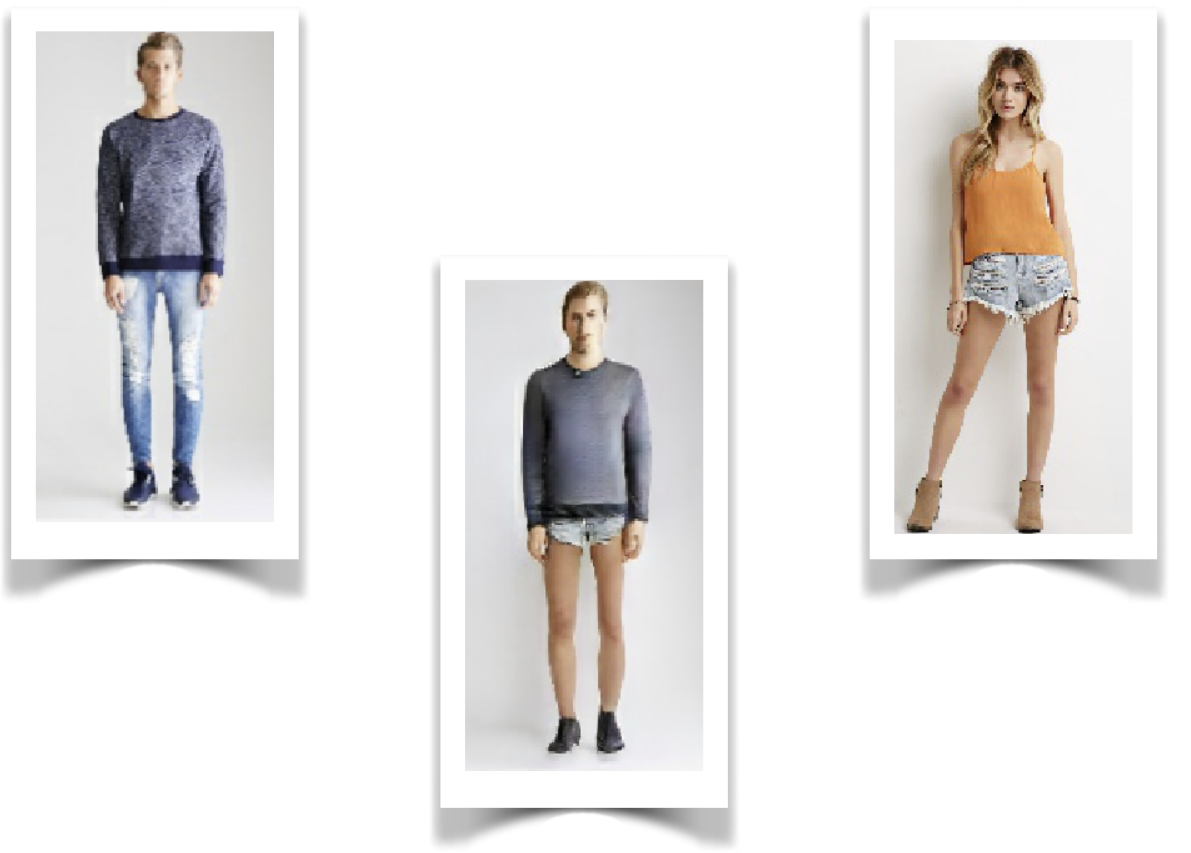
\includegraphics[trim={0cm 0cm 0cm 0cm},clip, width=0.4\linewidth]{fig/other/hotpants}
		\caption{\textit{"Imagine, how ridiculous you would look if you wore that hot pants"} - Thought experiments are a targeted manipulation of a disentangled representation.}
		\label{fig:hotpants}
	\end{figure}
\end{frame}

\begin{frame}
\frametitle{How Not to Disentangle.}
	\begin{figure}[htp]
		\centering
		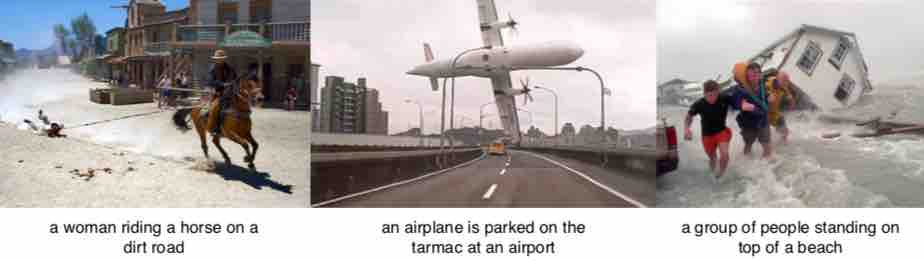
\includegraphics[trim={0cm 0cm 0cm 0cm},clip, width=1.\linewidth]{fig/other/notcausal}
		\caption{The image captions are generated by a deep neural network (Neuraltalk2) \cite{karpathy15neuraltalk}. Yet, common sense understanding of psychological and physical entities in terms of causal relationships and narratives is absent \cite{tenenbaum18think}. Instead, the neural network seems to capture mere associations.}
		\label{fig:notcausal}
	\end{figure}
\end{frame}

\begin{frame}
\frametitle{How can Humans Disentangle?}
	\begin{itemize}
		\item Priors:
		\item Data: temporal and interventional
		\note{image of child which destroys something}
		\item Models
	\end{itemize}
\end{frame}

\begin{frame}
\frametitle{Contributions}
	\begin{itemize}
		\item  \textit{Hypothesis \emph{i)}: Unsupervised learning of object shape benefits from abstracting away the complement of shape, namely the object appearance. Explaining away the appearance factor can be achieved by a disentangled generative modelling of both factors.}
		\item \textit{Hypothesis \emph{ii)}: Learning unsupervised disentanglement without any assumptions is fundamentally impossible. In accordance with the literature on causal learning, % \cite{pearl18impediments}
		disentangling causal factors requires model assumptions and/or interactional data - instead of observational (raw) data.}
	\end{itemize}
\end{frame}

\begin{frame}[t]
\frametitle{Overview}
\tableofcontents
\end{frame}


\section{Prerequisites}
	\subsection{Learning Disentangling Representations}
	\subsection{Impediments from Causality}

\section{Disentangling by Transforming}
	\begin{frame}
	\frametitle{Disentangling by Transforming}
		\begin{figure}[t]
			\centering
			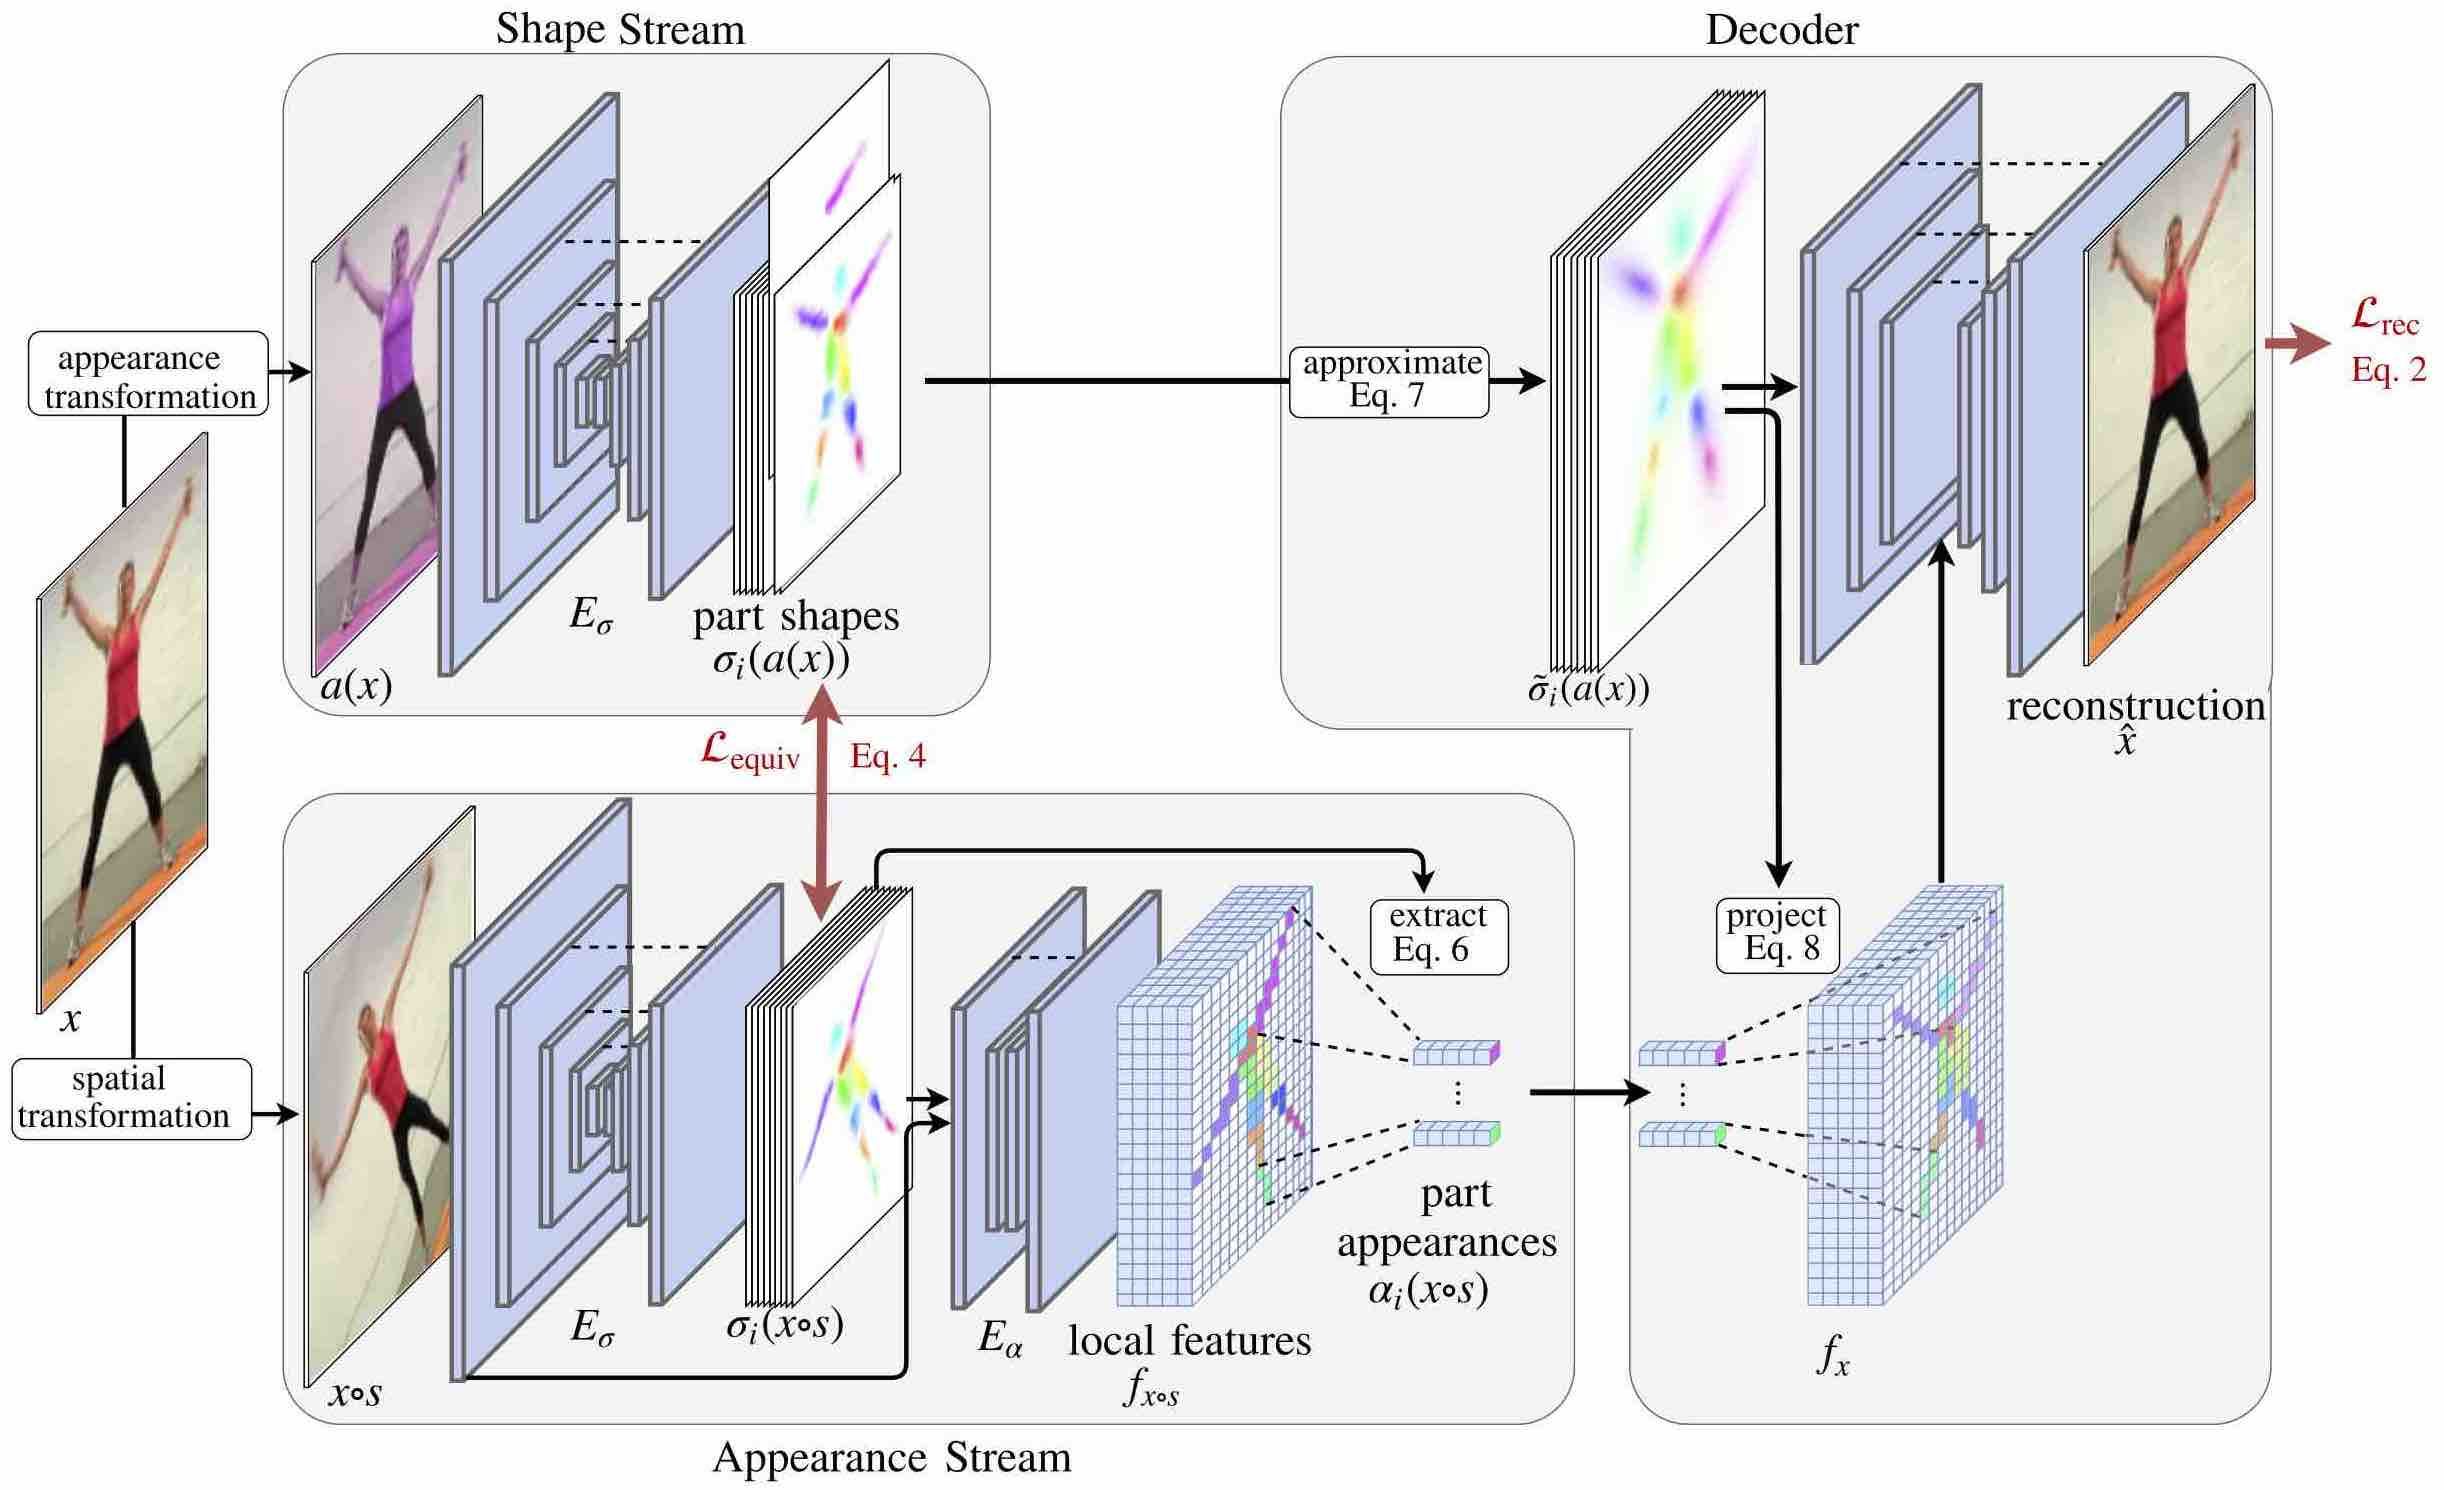
\includegraphics[trim={0cm 0cm 0cm 0cm},clip, width=1.\linewidth]{fig/other/architecture_final}
			\caption{Encoder $E$ encodes shape and appearance for two transformed images $s(\mathbf{x})$ and $a(\mathbf{x})$, after recombination $R$ of $({\alpha}_{s(\mathbf{x})}, {\sigma}_{a(\mathbf{x})})$ into latent image $Z$, the decoder $D$ reconstructs the image $\mathbf{x}$.}
			\label{fig:architecture}
		\end{figure}
	\end{frame}

	\begin{frame}
	\frametitle{Invariance and Equivariance}
		\begin{align}
			{\alpha}_{s(\mathbf{x})}  &= {\alpha}_{\mathbf{x}} \tag{invariance of appearance}\\
			{\sigma}_{a(\mathbf{x})} &= {\sigma}_{\mathbf{x}}  \tag{invariance of shape}\\
			{\sigma}_{s(\mathbf{x})} &= s({\sigma}_{\mathbf{x}}) \tag{equivariance of shape}
		\label{eq:invar}
		\end{align} % quad \forall i \leq n
	\end{frame}

	\begin{frame}
	\frametitle{Objective}
		\begin{equation}\label{eq:loss_rec}
			\mathcal{L}_{\textrm{rec}}= \lVert  \mathbf{x}  - \mathrm{D}[{\alpha}_{s(\mathbf{x})}, {\sigma}_{a(\mathbf{x})}]\rVert
		\end{equation}

		\begin{equation}
			\mathcal{l}_{\textrm{equiv}}^i = \mathcal{l}_{\mu}^i+ \mathcal{l}_{\sigma}^i
		\label{covariance}
		\end{equation}
		The overall loss objective is the sum of the reconstruction loss and the equivariance loss for all $n$ parts:
		\begin{equation}
		\mathcal{L} = \sum_{i=1}^n \mathcal{L}_{\text{equiv}}^i + \mathcal{L}_{\textrm{rec}}
		\end{equation}
	\end{frame}


\section{Object Shape Learning}
		\begin{frame}
		\frametitle{Learned Shapes}
			% PENN SHAPES
			\begin{figure}[htp]
				\begin{subfigure}{1.\textwidth}
				\centering
				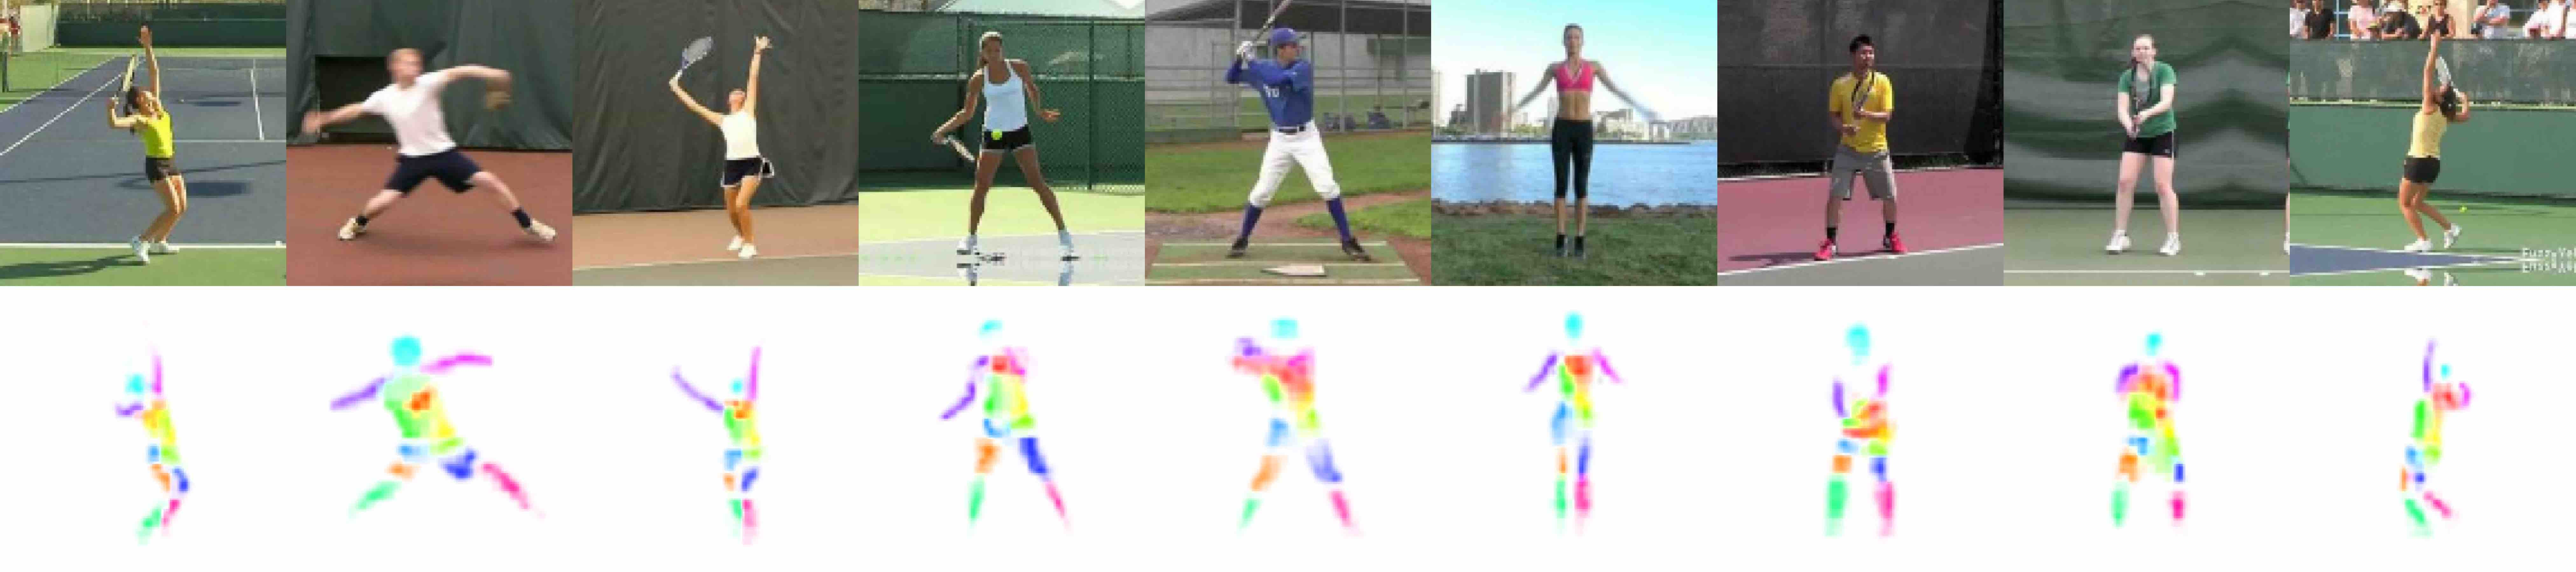
\includegraphics[trim={0cm 0cm 0cm 0cm},clip, width=1.\linewidth]{fig/shape/shape8white}\caption{}
				\label{fig:shape_penn}
				\end{subfigure}
				\begin{subfigure}{1.\textwidth}
				\centering
				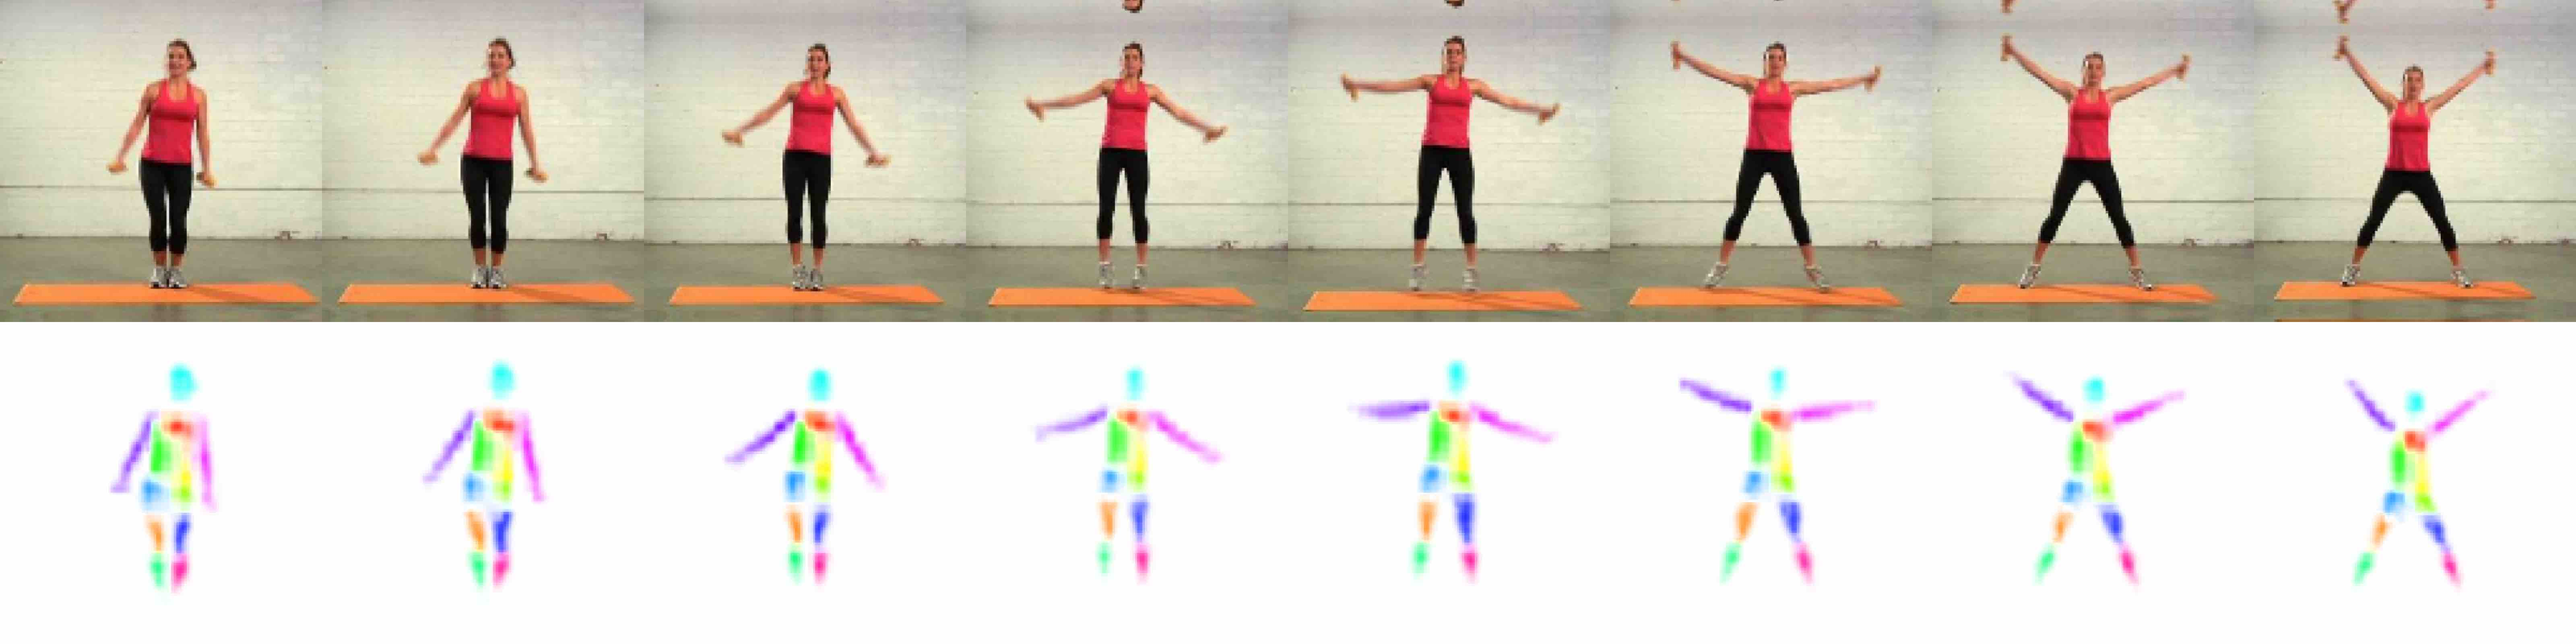
\includegraphics[trim={0cm 0cm 0cm 0cm},clip, width=1.\linewidth]{fig//shape/shape_yoga8}\caption{}
				\label{fig:shape_tennis}
				\end{subfigure}
				\caption{Learned shape representation on Penn Action. For visualization, 13 of 16 part activation maps are plotted in one image. (a) Different instances, showing intra-class consistency and (b) video sequence, showing consistency and smoothness under motion, although each frame is processed individually.}
				\label{fig:shape}
			\end{figure}
		\end{frame}

		\begin{frame}
		\frametitle{Landmark Regression}
			\begin{itemize}
				\item Protocol from Thewlis
			\end{itemize}
		\end{frame}

	\subsection{Diverse Object Categories}
		\begin{frame}
		\frametitle{Human and Cat Faces}
			% FACES
			\begin{figure}[htp]
				\centering
				\begin{subfigure}{1.\textwidth}
				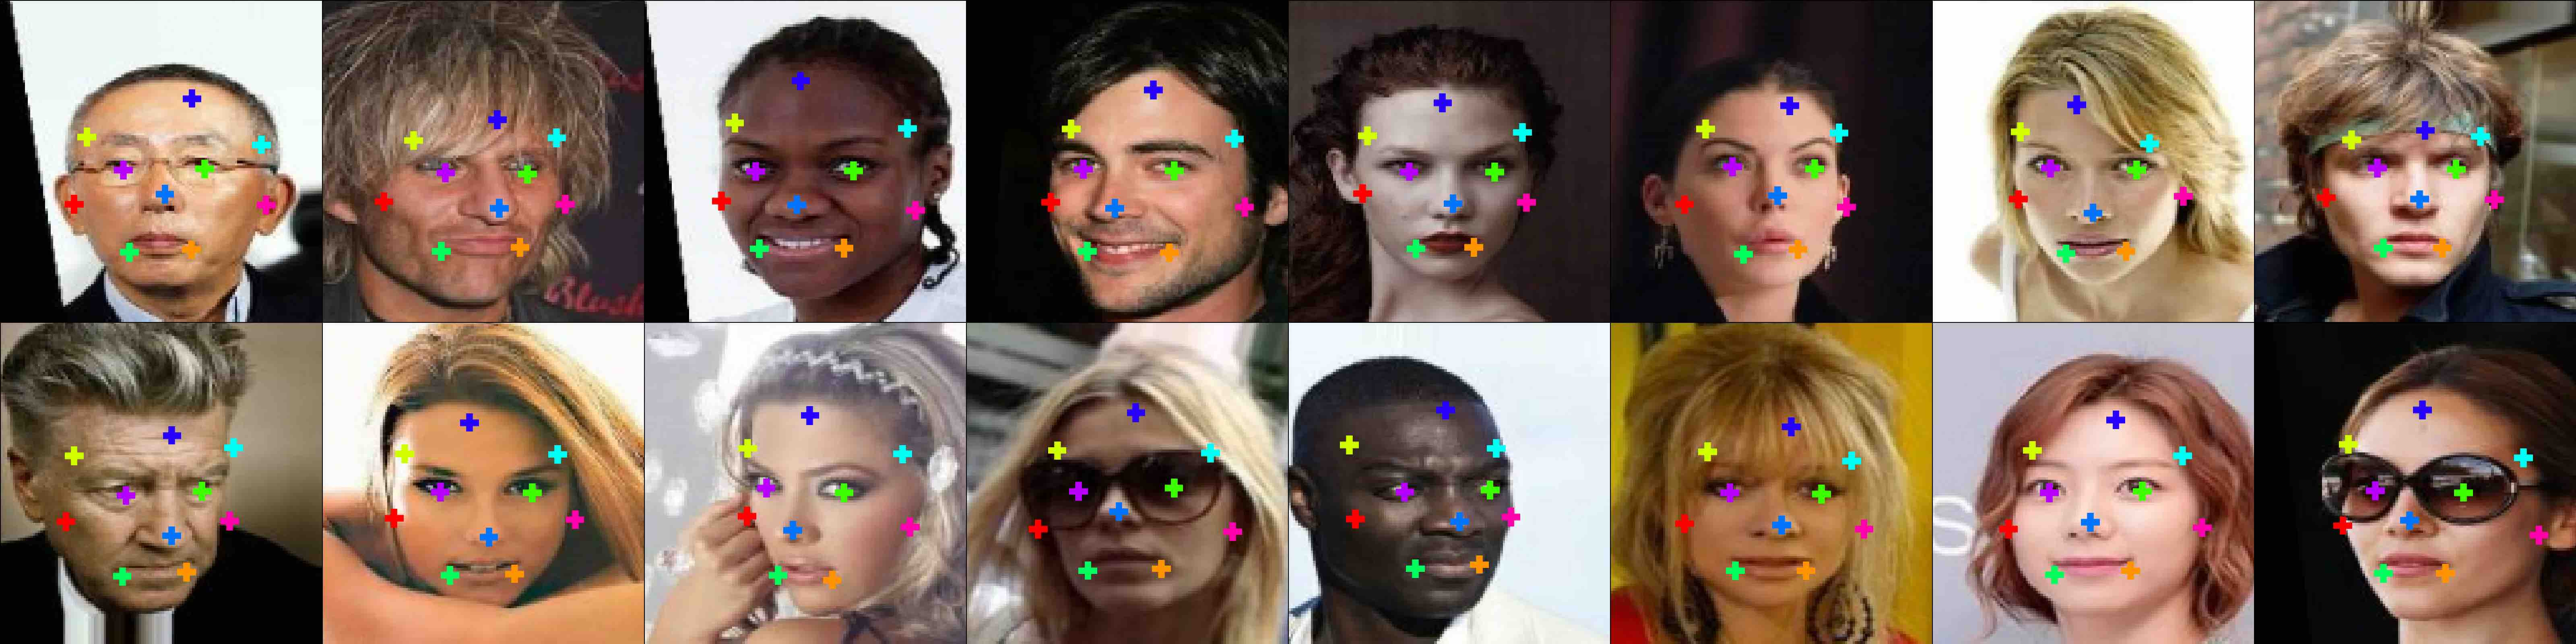
\includegraphics[trim={0cm 0cm 0cm 0cm},clip, width=1.\linewidth]{fig/shape/0celeba}\caption{}
				\end{subfigure}
				\begin{subfigure}{1.\textwidth}
				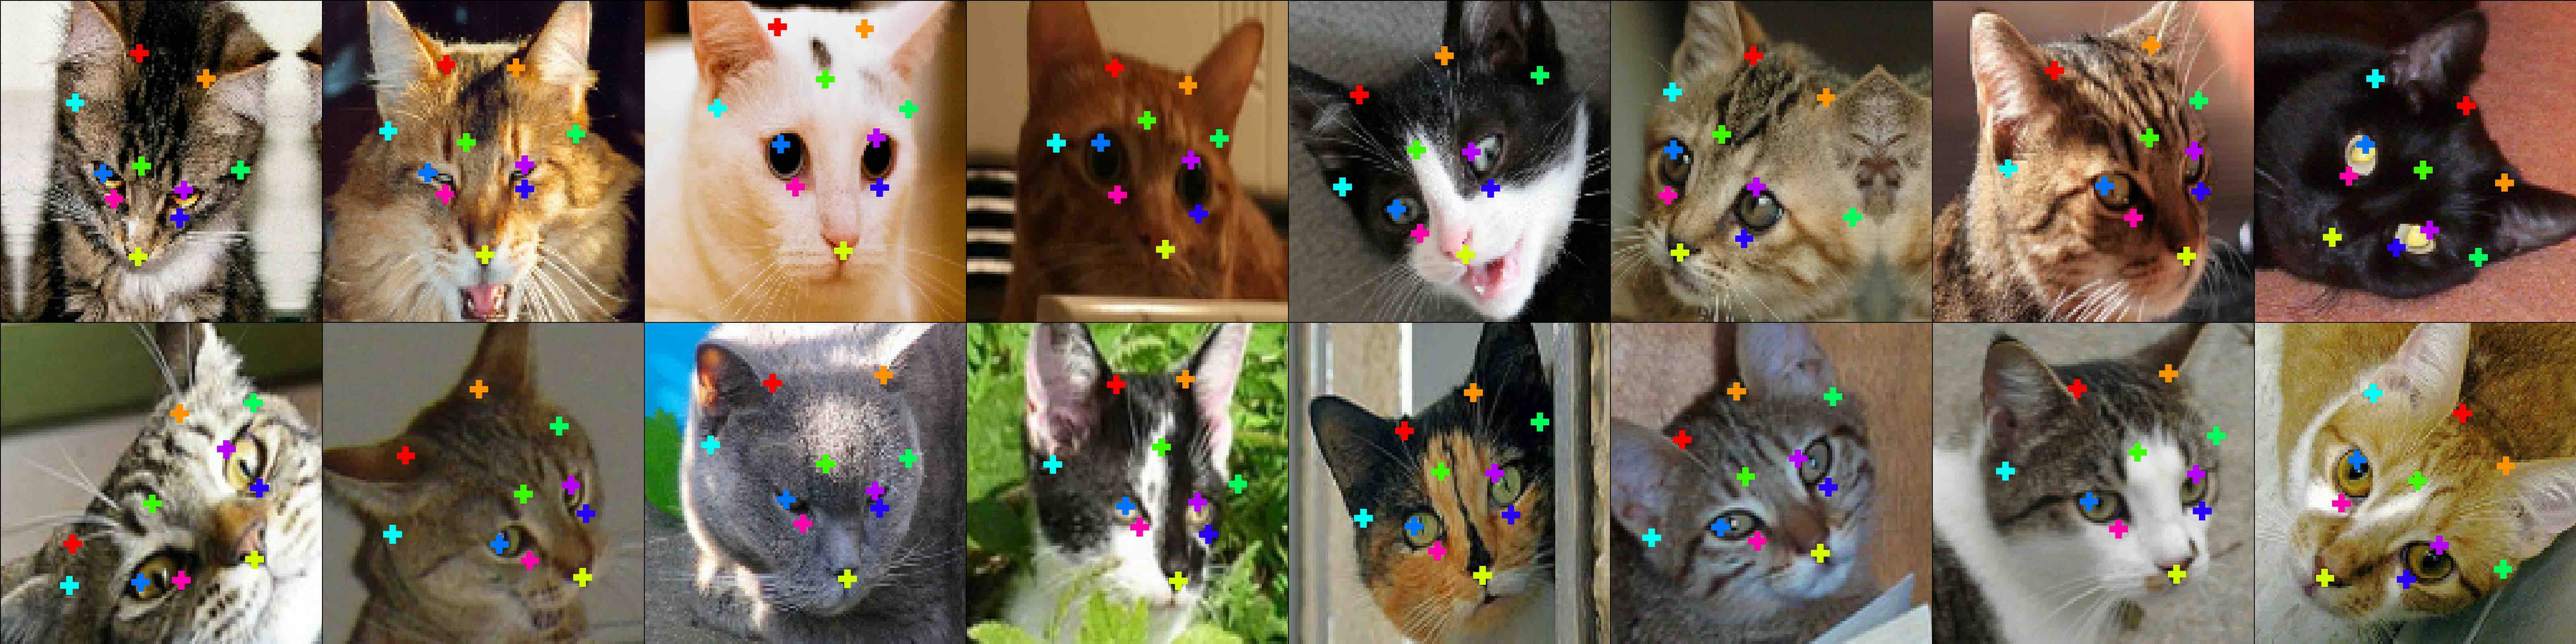
\includegraphics[trim={0cm 0cm 0cm 0cm},clip, width=1.\linewidth]{fig/shape/0cats}\caption{}
				\end{subfigure}
				\caption{{Unsupervised discovery of landmarks the object classes of (a) human (CelebA dataset) and (b) cat faces (Cat Head dataset).}}
				\label{fig:kp_faces}
			\end{figure}
		\end{frame}

		\begin{frame}[t]
		\frametitle{Human and Cat Faces}
			\begin{table}[t]
					\caption{Error of unsupervised methods for landmark prediction on the Cat Head, MAFL (subset of CelebA) testing sets. The error is in \% of inter-ocular distance.}
					\label{tab:faces}
					\centering
					\begin{tabular}{l|ccc}
					\hline
					Dataset & Cat Head &  & MAFL \\
					  \# Landmarks &10 & 20  & 10  \\
					  \hline
					 Thewlis \cite{thewlis17}
					 & 26.76 & 26.94 & 6.32    \\
					 Jakab \cite{jakab18}
					 & - & - & 4.69  \\
					 Zhang \cite{zhang18}
					 & 15.35 & 14.84 & 3.46  \\
					  Ours & \textbf{9.88}  & \textbf{9.30} & \textbf{3.24}  \\ \hline  % image length is 600: 32.15 , 23.51
					\end{tabular}
			\end{table}
		\end{frame}

		\begin{frame}[t]
		\frametitle{Human Bodies}
			\begin{figure}[htp]
				\centering
				\begin{subfigure}{1.\textwidth}
				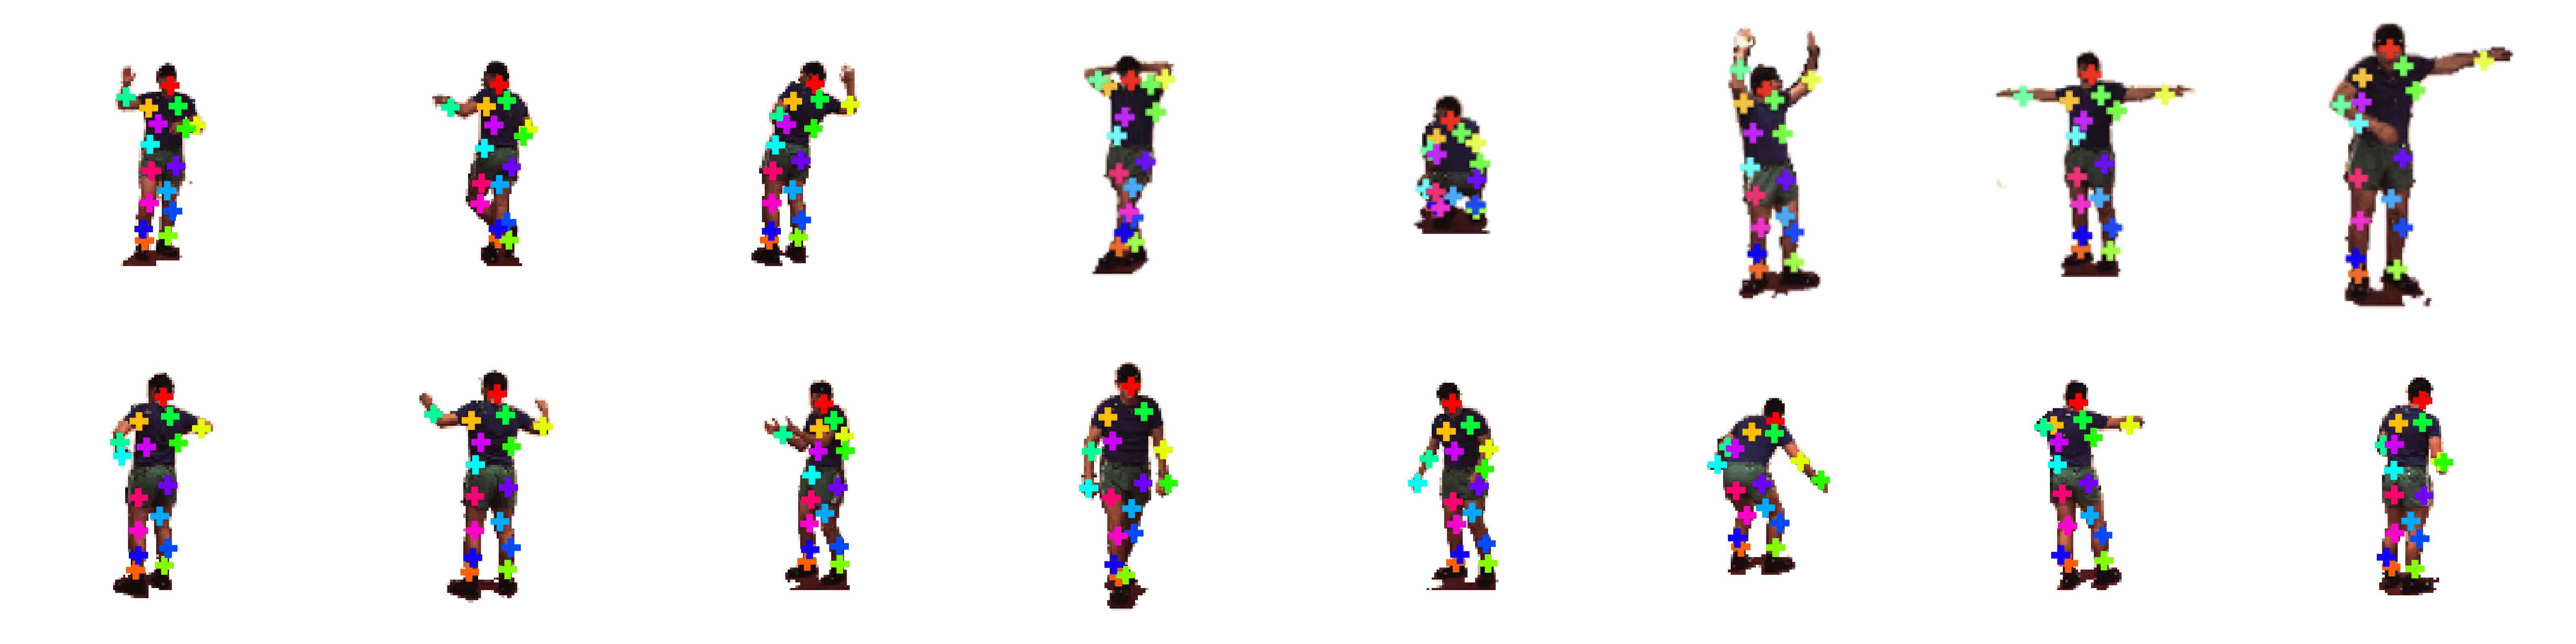
\includegraphics[trim={0cm 0cm 0cm 0cm},clip, width=1.\linewidth]{fig/shape/0human}\caption{}
				\end{subfigure}
				\begin{subfigure}{1.\textwidth}
				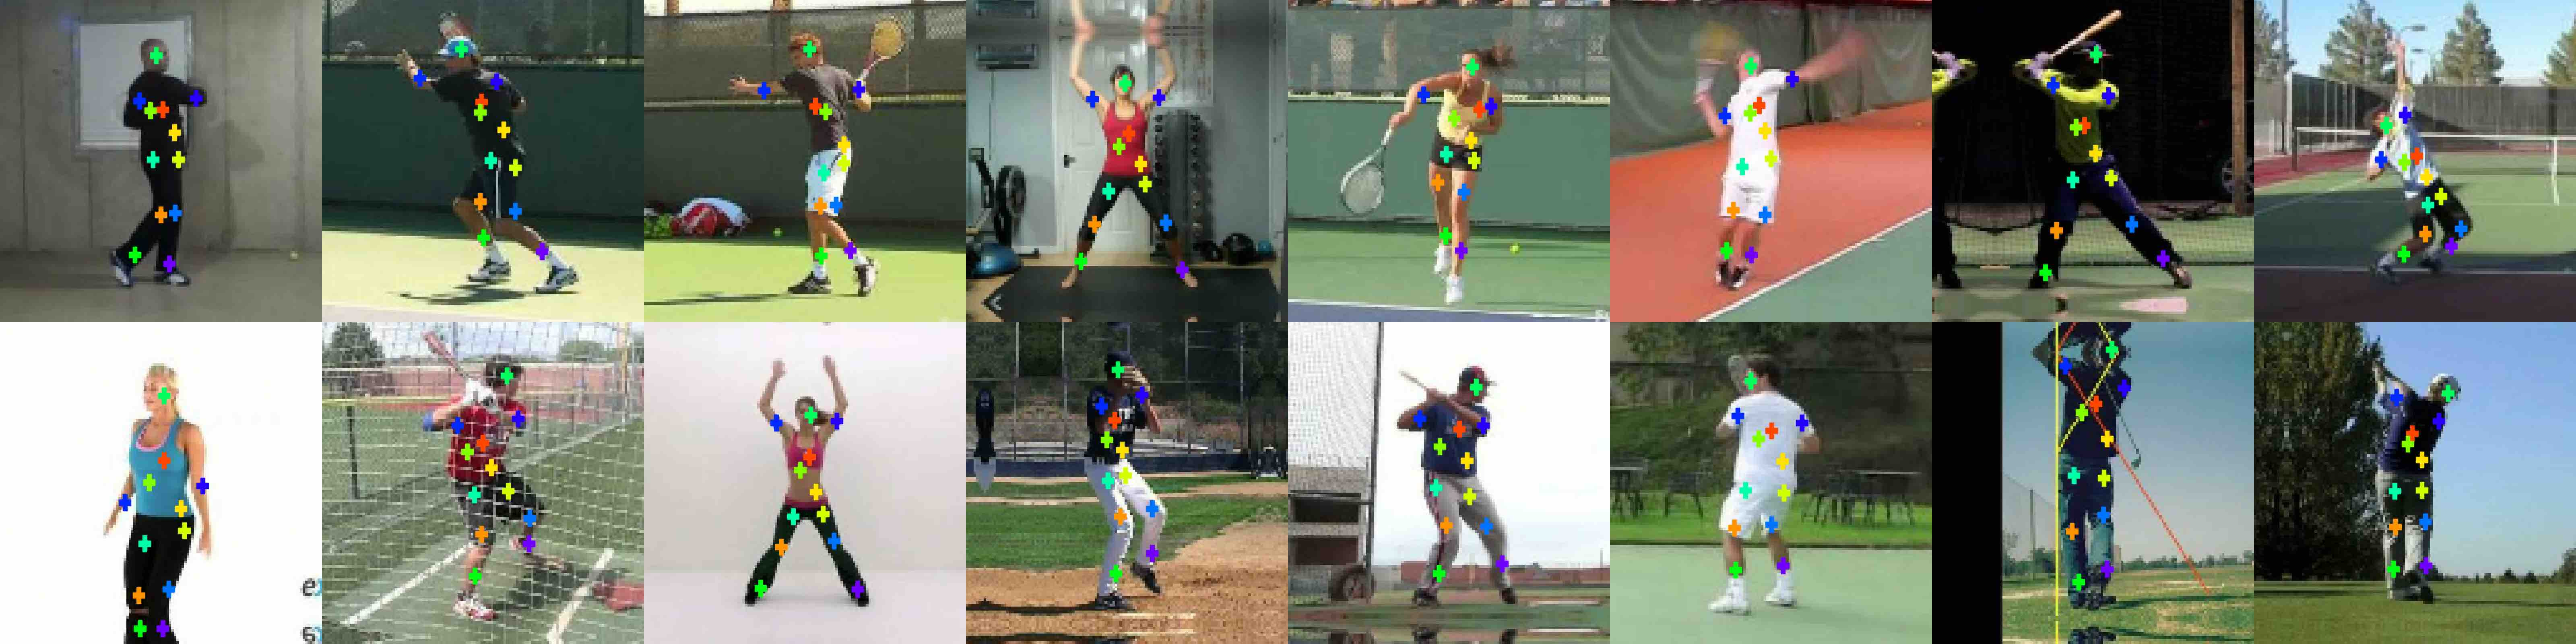
\includegraphics[trim={0cm 0cm 0cm 0cm},clip, width=1.\linewidth]{fig/shape/0penn}\caption{}
				\end{subfigure}
				\caption{{Unsupervised discovery of landmarks the object classes of human bodies (a) in constrained (Human3.6M dataset) and (b) unconstrained environments (Penn Action dataset).}}
				\label{fig:kp_bodies}
			\end{figure}
		\end{frame}

		\begin{frame}[t]
		\frametitle{Human Bodies}
			% BBC POSE Results
				\begin{table}[htp]
					\caption{{
					Performance of landmark prediction on BBC Pose test set. As upper bound, we also report the performance of supervised methods.
					%Comparing against supervised and unsupervised methods for annotated landmark prediction on the BBC Pose testing set.
					The metric is \% of points within 6 pixels of groundtruth location. %Note that Jakab et al. are using a 50-landmarks, while we only use a 30 landmarks as input for the regression.
					}}
					\label{tab:bbcpose}
					\centering
					\begin{tabular}{ll|cr}
					\hline
					BBC Pose &   &    { Accuracy}  \\
					 \hline
					supervised & Charles \cite{charles13bbcpose} &
					   79.9\%  \\ % 79.90
					 & Pfister \cite{pfister15flowingconv}  &
					  88.0\%  \\ \hline % 88.01
					unsupervised &Jakab \cite{jakab18} &
					 68.4\%  \\  % 68.44
					  &Ours &  \textbf{74.5}\% \\
					% test pck = 0.7484605918670523
					% test pck_per_kp = [0.9633621  0.6627155  0.76508623 0.54956895 0.6928879  0.76616377   0.83943963]
					\hline
					\end{tabular}
				\end{table}

				% HUMAN3.6M Results
				\begin{table}[htp]
					\caption{{Comparing against supervised, semi-supervised and unsupervised methods for landmark prediction on the Human3.6M test set. The
					error is in \% of the edge length of the image. All methods predict 16 landmarks.
					}}
					\label{tab:human}
					\centering
					\begin{tabular}{ll|cr}
					\hline
					 Human3.6M   & &  { Error w.r.t. image size}  \\
					 \hline
					 supervised & Newell \cite{newell16hourglass}
					  &2.16  \\  \hline
					 semi-supervised & Zhang \cite{zhang18}
					  & 4.14  \\ \hline
					 unsupervised & Thewlis \cite{thewlis17}
					 & 7.51  \\
					  & Zhang \cite{zhang18}
						& 4.91 \\
					  & Ours& \textbf{2.79} \\
					\hline
					\end{tabular}
				\end{table}
		\end{frame}

		\begin{frame}[t]
		\frametitle{Animal Bodies}
			\begin{figure}[htp]
				\centering
				\begin{subfigure}{1.\textwidth}
				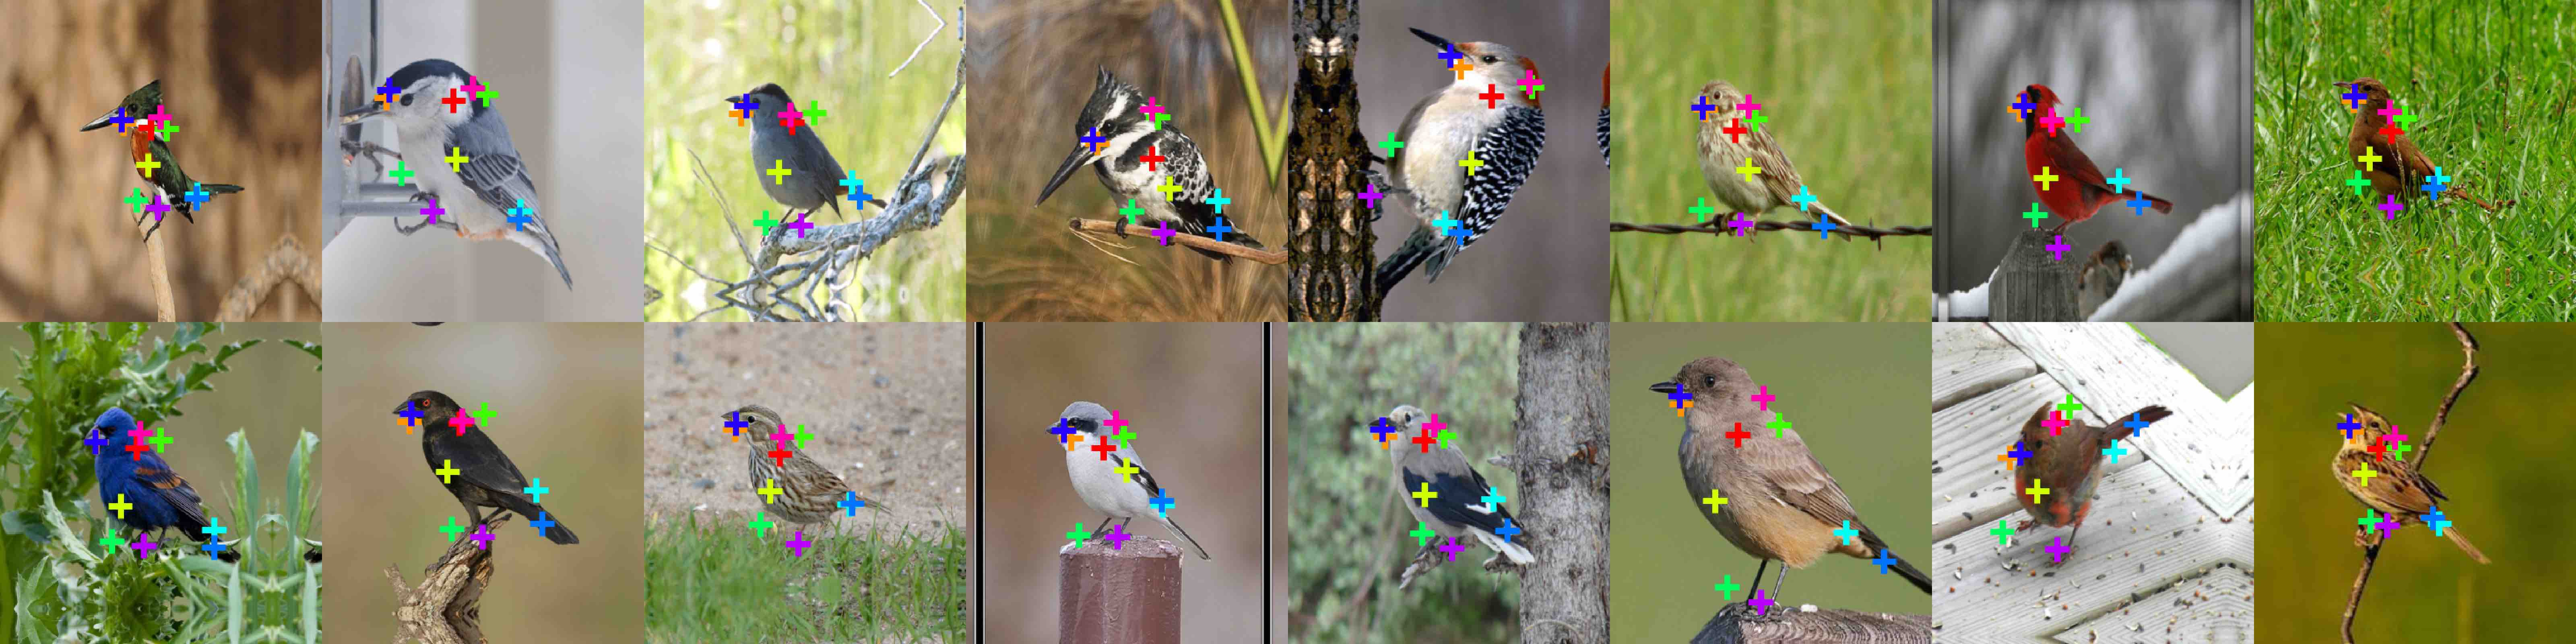
\includegraphics[trim={0cm 0cm 0cm 0cm},clip, width=1.\linewidth]{fig/shape/0birds}\caption{}
				\end{subfigure}
				\begin{subfigure}{1.\textwidth}
				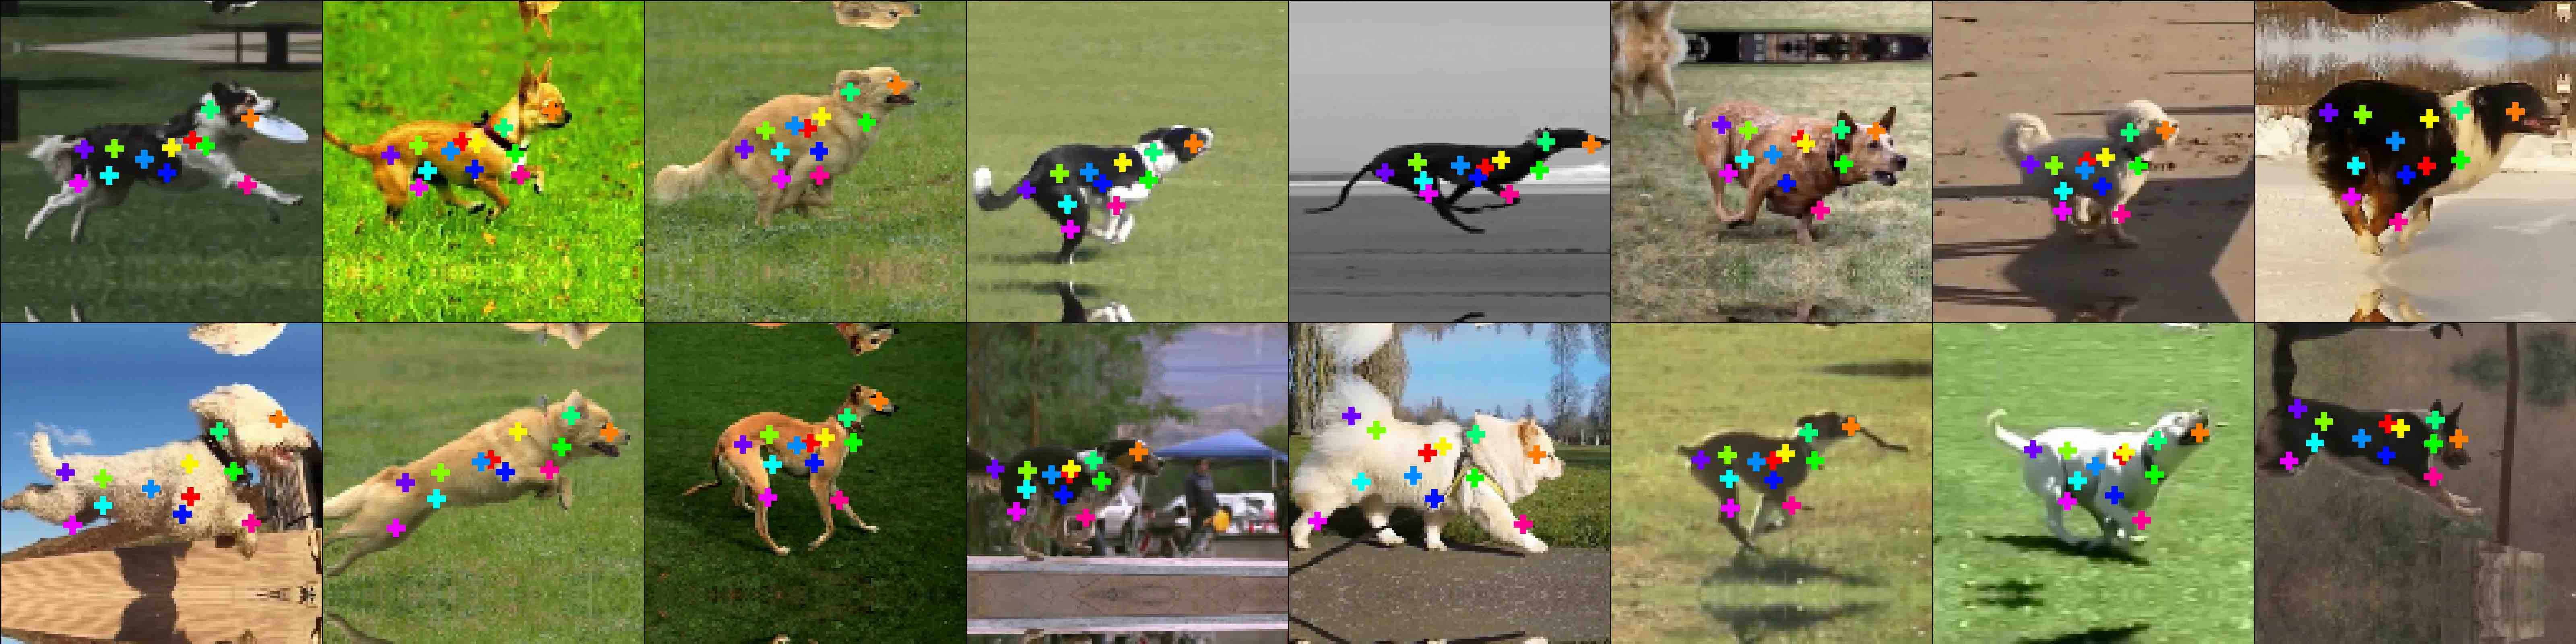
\includegraphics[trim={0cm 0cm 0cm 0cm},clip, width=1.\linewidth]{fig/shape/0dogs}\caption{}
				\end{subfigure}
				\caption{{Unsupervised discovery of landmarks the object classes of animal bodies (a) birds (CUB-200-2011 dataset) and (b) dogs (Dogs Run dataset).}}
				\label{fig:kp_animals}
			\end{figure}
		\end{frame}

		\begin{frame}[t]
		\frametitle{Animal Bodies}
			% RESULTS BIRDS
			\begin{table}[t]
				\caption{Error of unsupervised methods for landmark prediction on the CUB-200-2011 testing set. Both methods predict 10 landmarks.}
				% The error is in \% of edge length of the image.}
				\label{tab:birds}
				\centering
				\begin{tabular}{l|cccc}
					\hline
					CUB-200-2011 dataset&  & Error \wrt image edge\\
					% \# Landmarks & 10  \\
					\hline
					Zhang \cite{zhang18} & 5.36 \\
					Ours  & \textbf{3.91}  \\ \hline
				\end{tabular}
			\end{table}
		\end{frame}

	\subsection{Challenges}
		\begin{frame}[t]
		\frametitle{Challenges}
			\begin{table}
				\centering
				\caption{Difficulties of datasets: articulation, intra-class variance, background clutter and viewpoint variation}
				\label{tab:challenges}
				\begin{tabular}{l|rrrr}
					\hline
					Dataset &  Articul.& Var. &  Backgr.& Viewp.  \\ \hline
					CelebA &   &  &  &    \\
					Cat Head & &  \checkmark&  &   \\
					CUB-200-2011 & & \checkmark& \checkmark&   \\
					Human3.6M &\checkmark& &  & \checkmark  \\
					BBC Pose &  \checkmark&  & \checkmark&  \\
					Dogs Run & \checkmark& \checkmark& \checkmark&   \\
					Penn Action & \checkmark& \checkmark& \checkmark& \checkmark  \\
					\hline
				\end{tabular}
			\end{table}
		\end{frame}

		\begin{frame}[t]
		\frametitle{Challenges}
			\begin{itemize}
				\item Background
				\item Articulation
				\item Viewpoint
				\item Intra-Class
			\end{itemize}
		\end{frame}

	\subsection{Transformations}
		\begin{frame}[t]
		\frametitle{Transformational Effects}
			\begin{figure}[htp]
				\begin{subfigure}{0.40\linewidth}
					\centering
					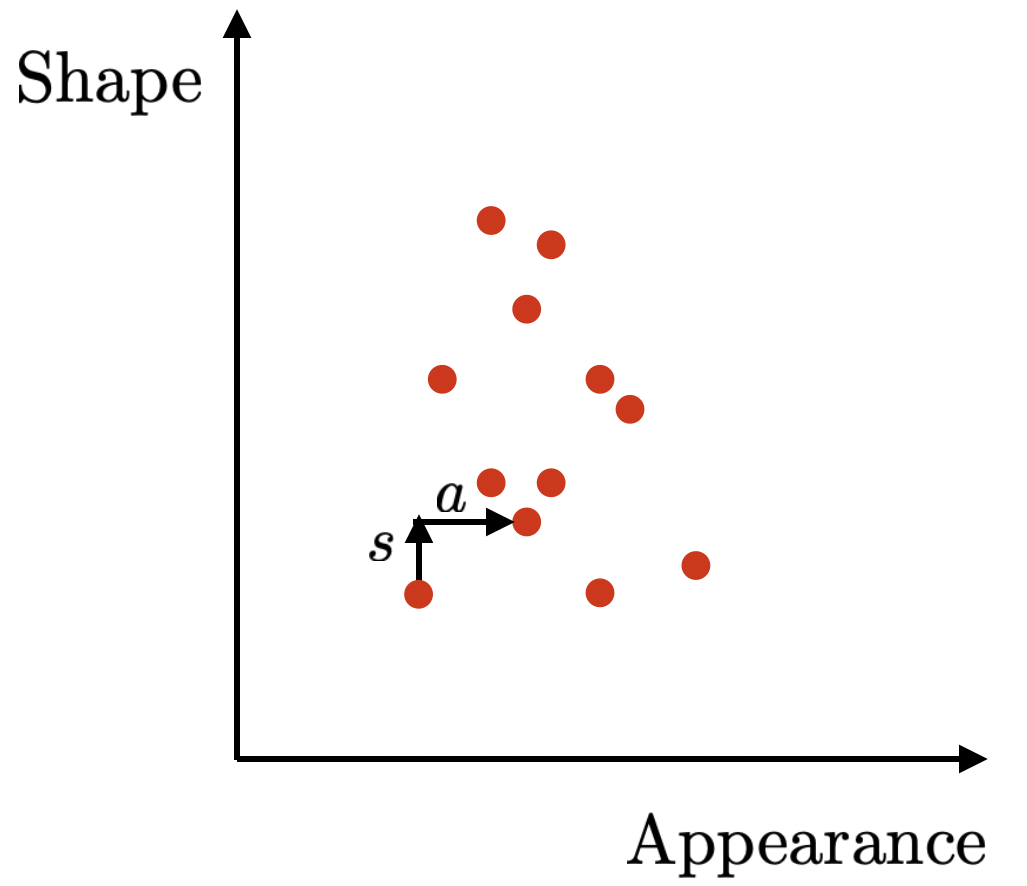
\includegraphics[trim={0cm 0cm 0cm 0cm},clip, width=1.\linewidth]{fig/other/trans}
					\caption{}
				\end{subfigure}
				\begin{subfigure}{0.40\linewidth}
					\centering
					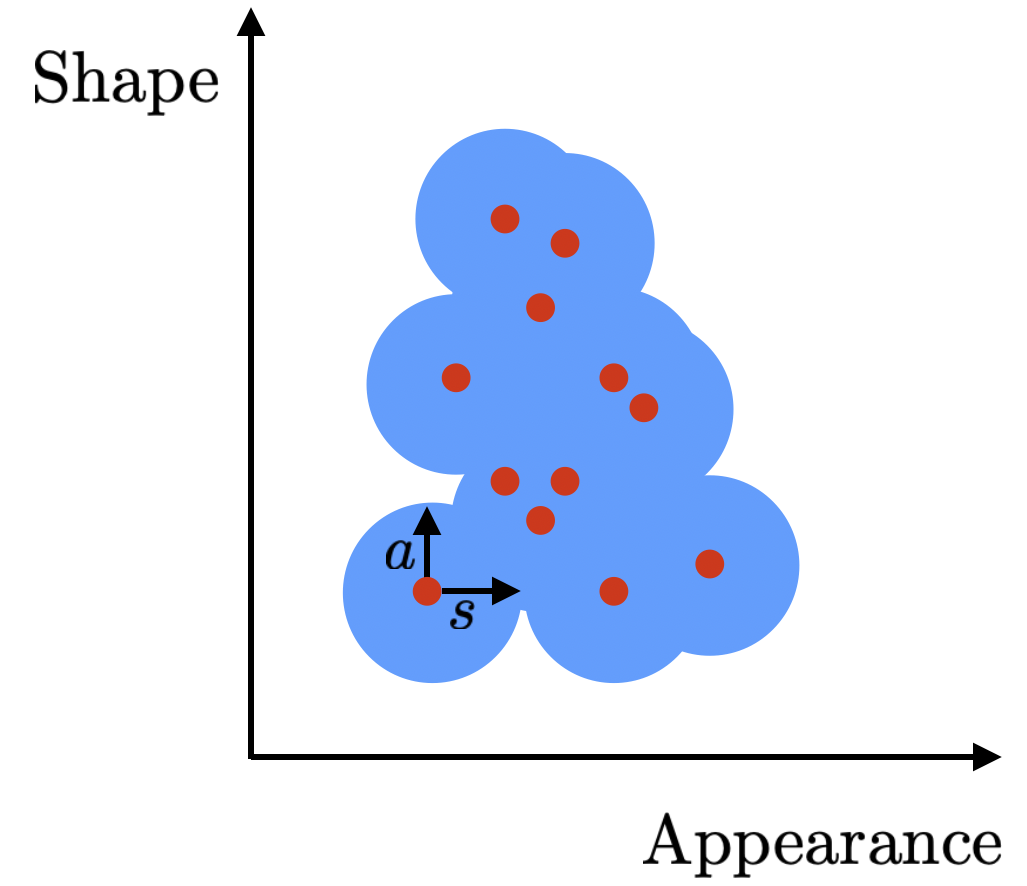
\includegraphics[trim={0cm 0cm 0cm 0cm},clip, width=1.\linewidth]{fig/other/trans2}
					\caption{}
				\end{subfigure}
				\caption{Effect of transformations on data distribution: (a) Data points (red) can be connected via a shape $s$ and an appearance $a$ transformation. (b) Applying transformations effectively blurs the data distribution.}
				\label{fig:trans}
			\end{figure}
		\end{frame}

		\begin{frame}[t]
		\frametitle{Shape and Appearance}
			% COLOR
			\begin{figure}[htp]
				\centering
				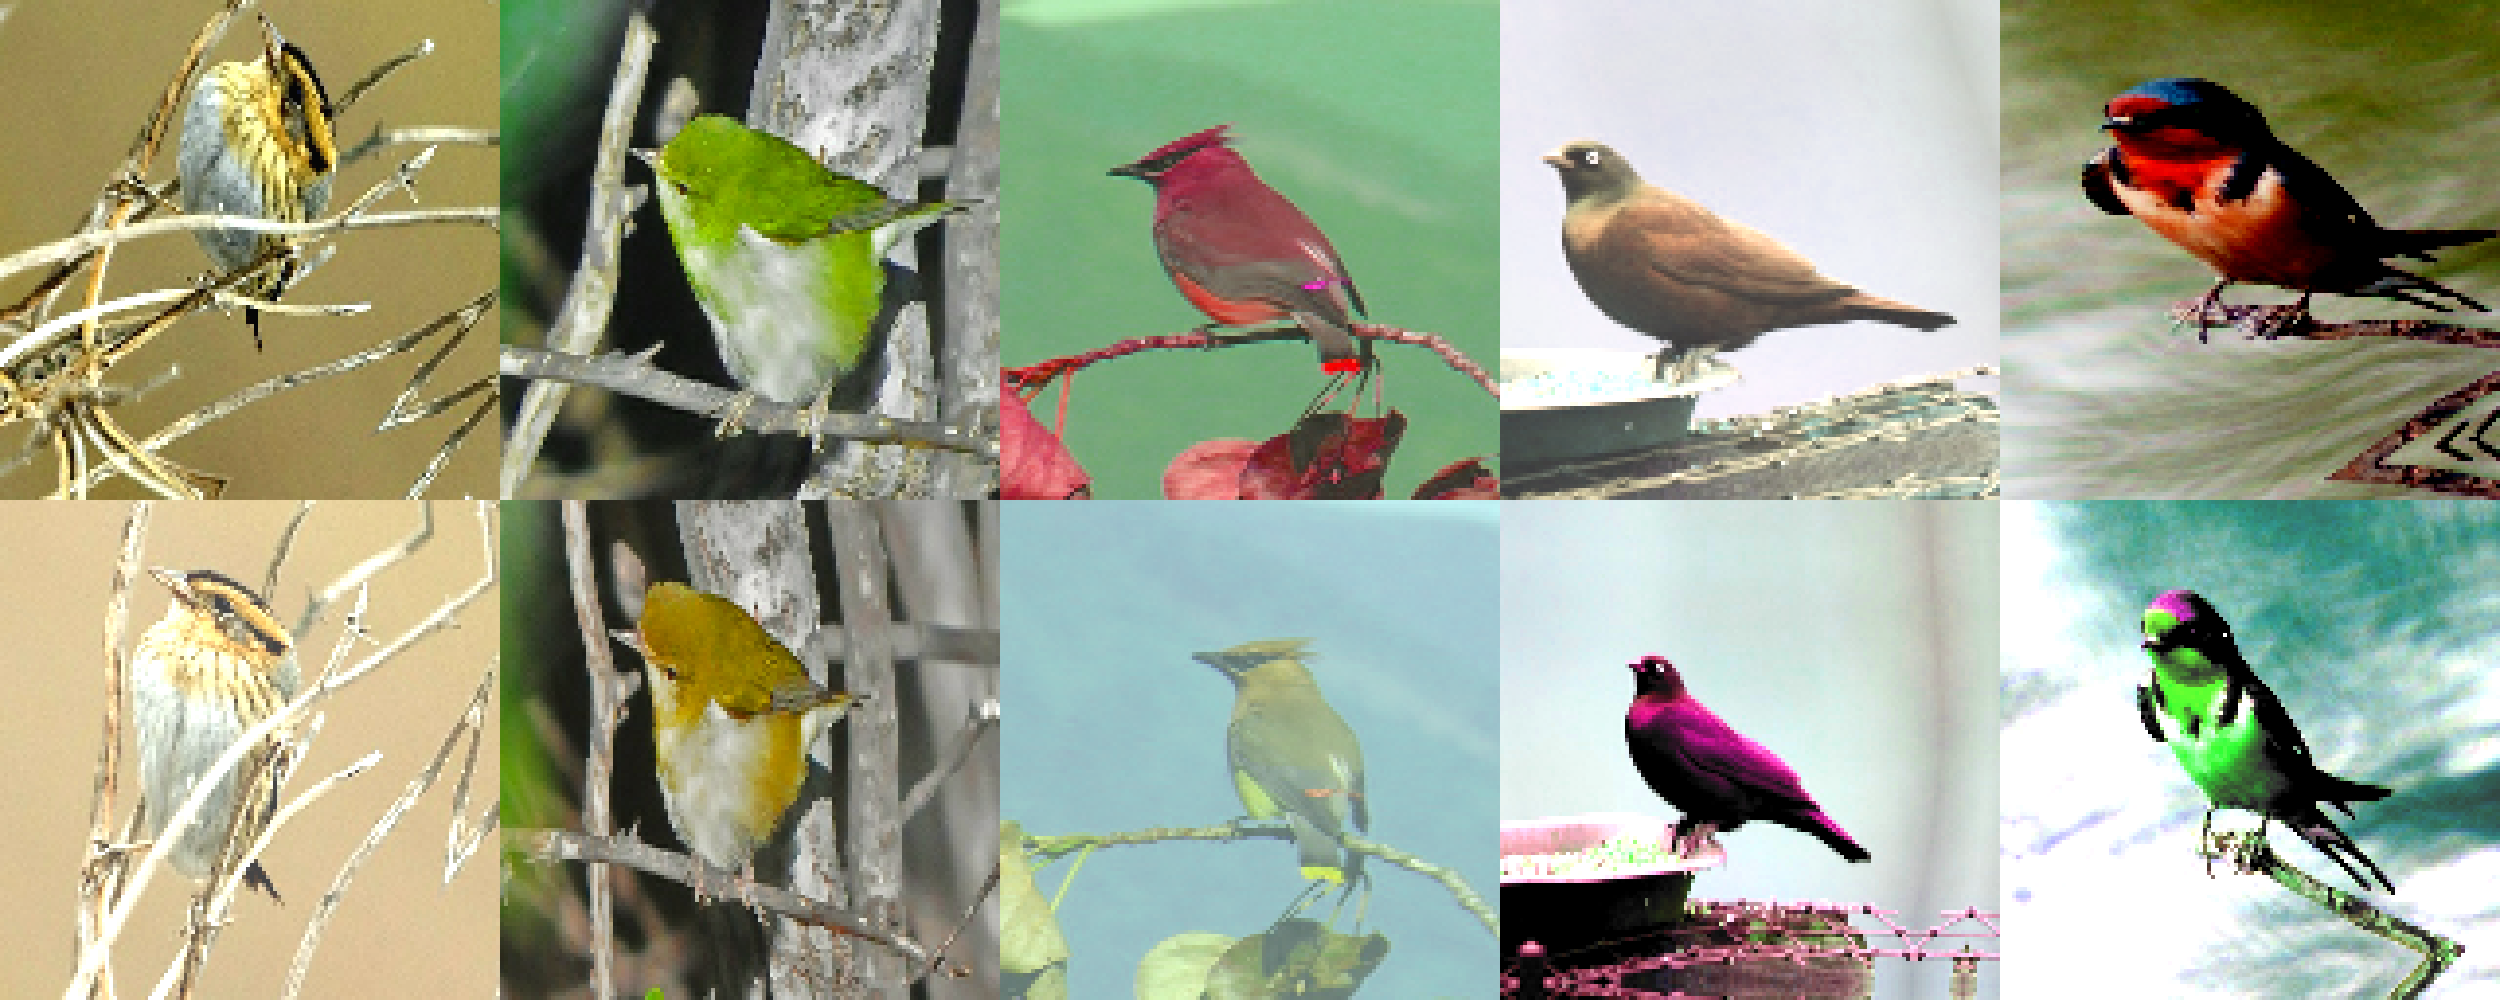
\includegraphics[trim={0cm 0cm 0cm 0cm},clip, width=.8\linewidth]{fig/shape/coloraugm}
				\caption{Examples for shape and appearance transformation on CUB-200-2011. Images from the upper row relate to images directly below.}
				\label{fig:coloraugm}
			\end{figure}
		\end{frame}

		\begin{frame}[t]
		\frametitle{Parity}
			\begin{figure}[htp]
				\centering
				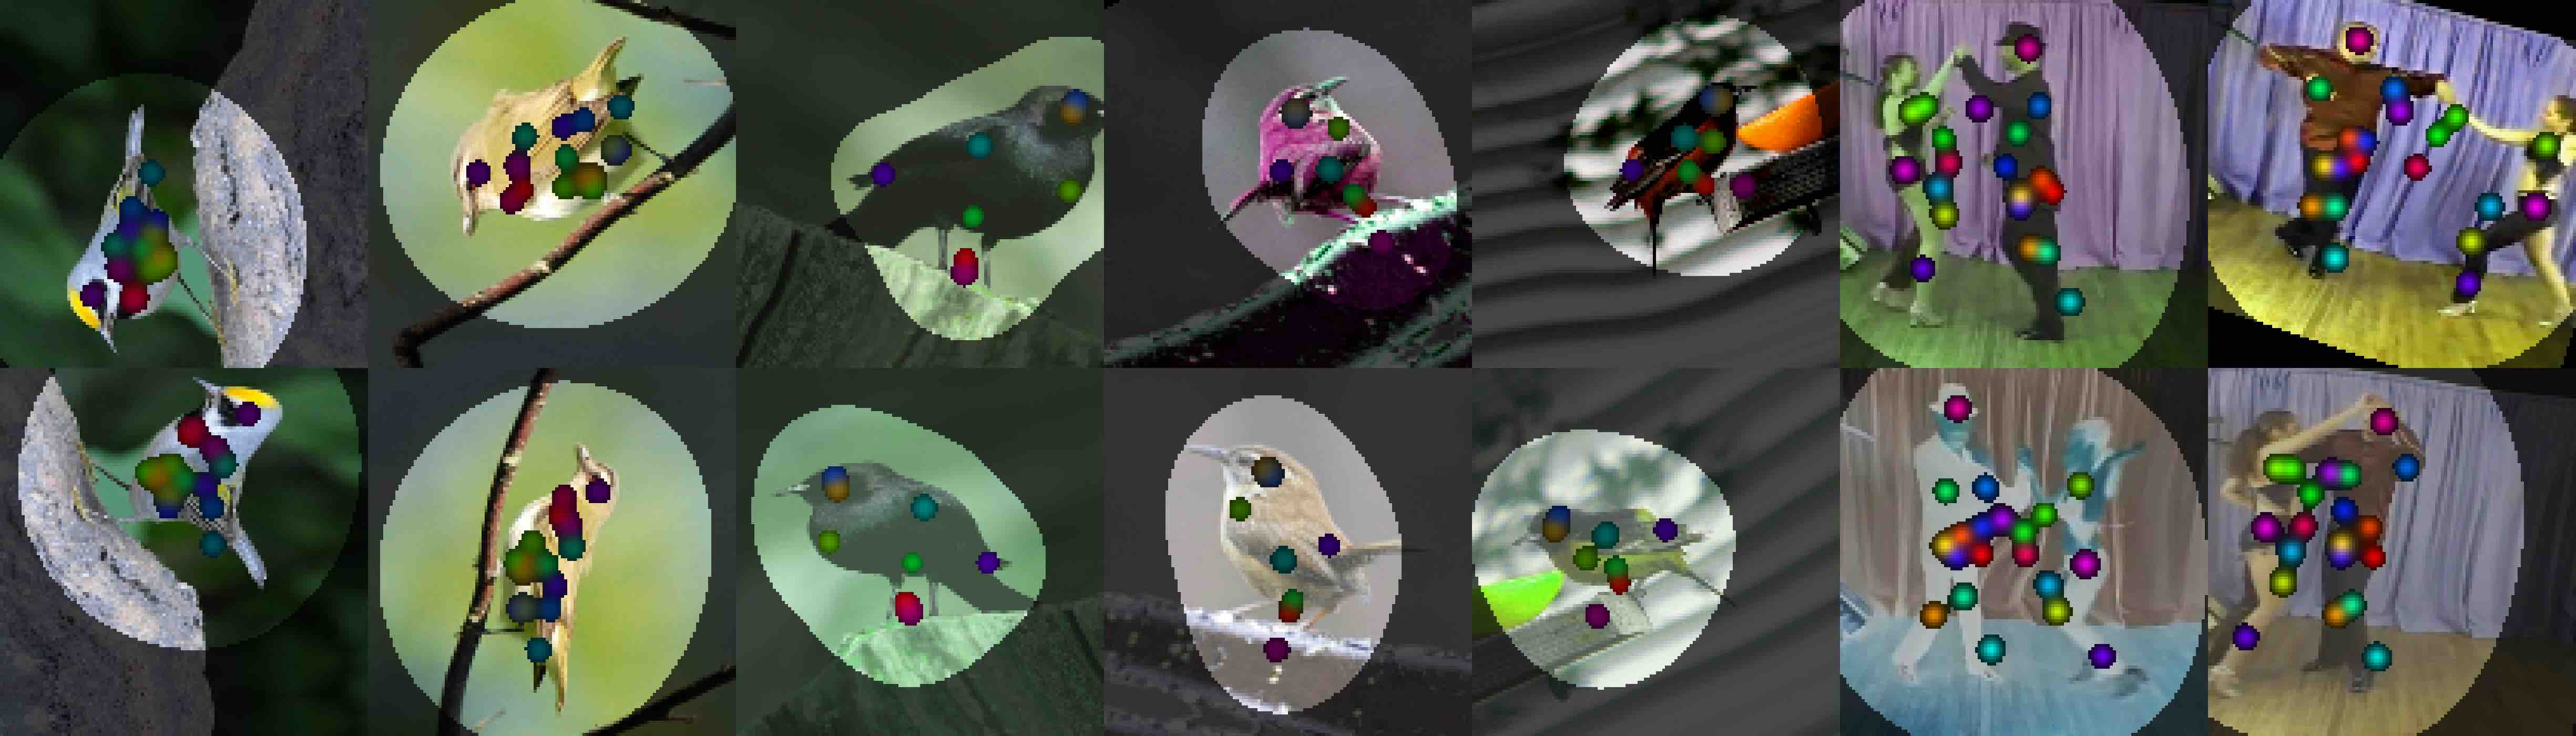
\includegraphics[trim={0cm 0cm 0cm 0cm},clip, width=1.\linewidth]{fig/shape/parity}
				\caption{Parity changes: the images of the upper and lower row relate via the usual transformations and an additional parity flip. For the bird (1-5th column) images induced artificially, for the dancing humans (6-7th column) via sampling different frames from a video.}
				\label{fig:parity}
			\end{figure}
		\end{frame}

	\subsection{Comparative Advantages}
		\begin{frame}[t]
		\frametitle{Non-Disentangling Approach}
			% COMPARE ZHANG
			\begin{figure}[htp]
				\centering
				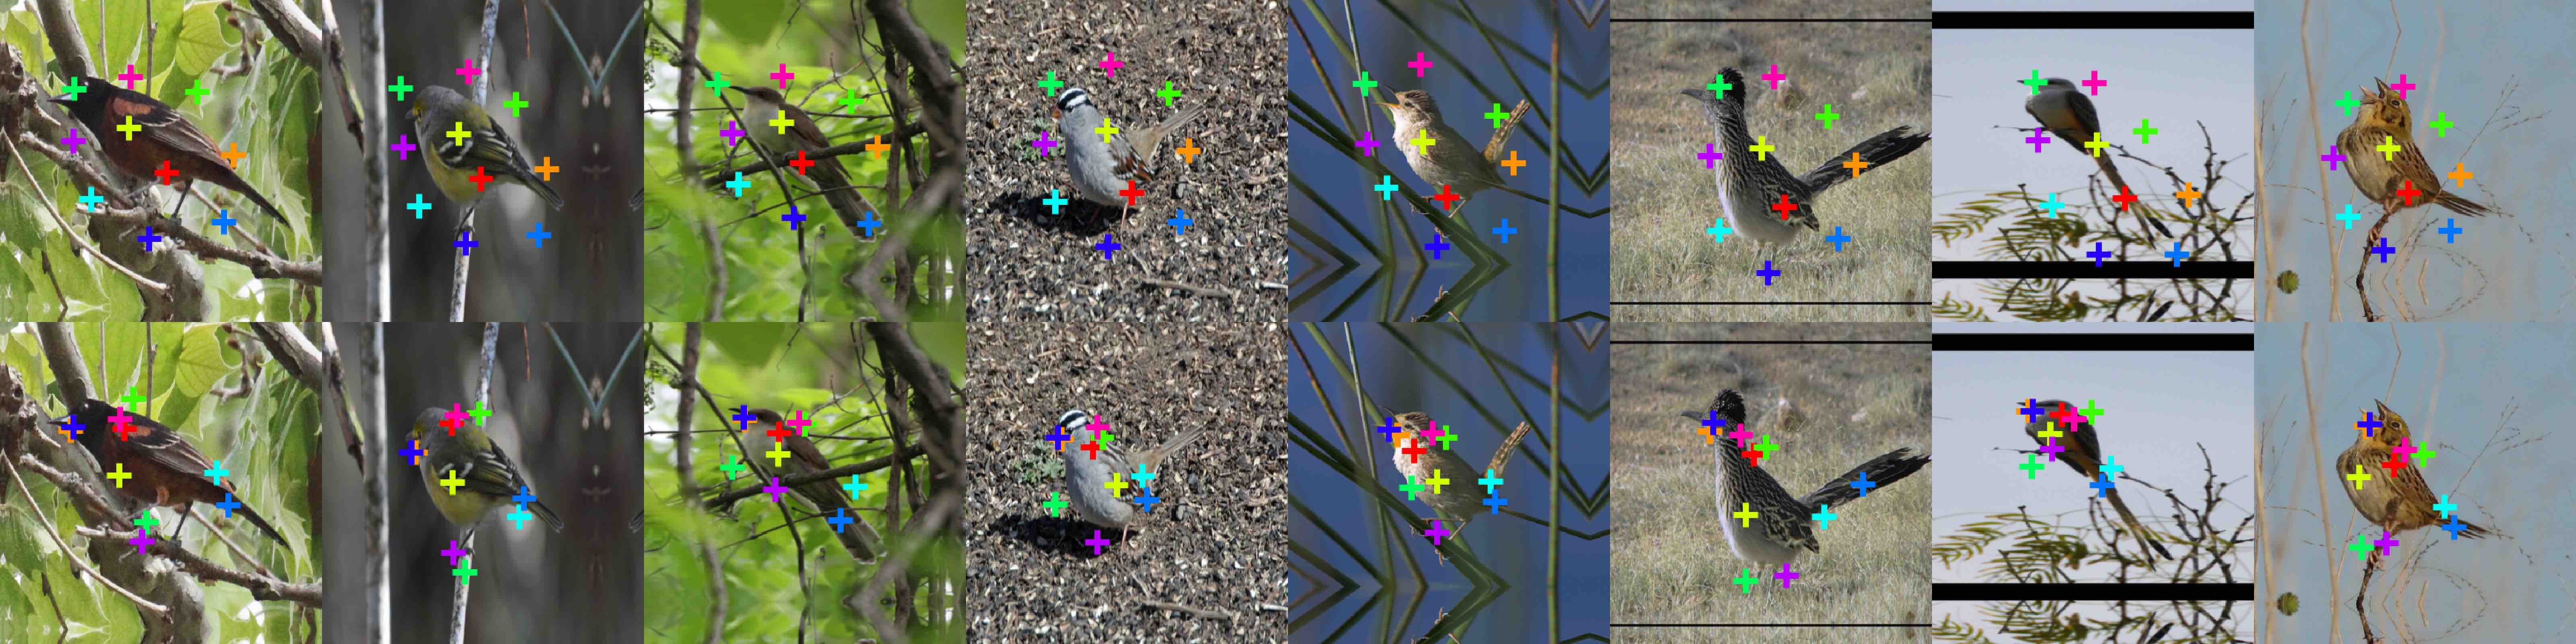
\includegraphics[trim={0cm 0cm 0cm 0cm},clip, width=1.\linewidth]{fig/shape/comp}
				\caption{Comparing discovered keypoints against \cite{zhang18} on CUB-200-2011. We improve on object coverage and landmark consistency. Note our flexible part placement compared to a rather rigid placement of \cite{zhang18} due to their part separation bias.}
				\label{fig:compare}
			\end{figure}
		\end{frame}

		\begin{frame}[t]
		\frametitle{Holistic Approach}
			% BBCPOSE DETAILED RESULTS
			\begin{table}[htp]
				\centering
				\begin{tabular}{l|ccccccr}
				\hline
				Dataset & BBCPose &  &  &  & &  &  \\
				Landmarks & {\footnotesize Head} & {\footnotesize Wrists} &  {\footnotesize Elbows }& {\footnotesize Shoulders } & {\footnotesize Avg.}  \\
				\hline
				Charles et al. \cite{charles13bbcpose}  (supervised)&
				95.40 & 72.95 & 68.70 & 90.30 & 79.90  \\
				Pfister et al.  \cite{pfister15flowingconv} (supervised) &
				98.00 & 88.45 & 77.10 & 93.50 & 88.01  \\ \hline
				Jakab \cite{jakab18}  (unsupervised) &
				76.10& 56.50& 70.70& 74.30 &68.44  \\
				Ours (unsupervised)  & \textbf{96.34} & \textbf{71.39} & \textbf{62.12} & \textbf{80.28}& \textbf{74.85} \\
				% test pck = 0.7484605918670523
				% test pck_per_kp = [0.9633621  0.6627155  0.76508623 0.54956895 0.6928879  0.76616377   0.83943963]
				\hline
				\end{tabular}
				\caption{{Comparison with supervised and unsupervised methods for annotated landmark prediction on the BBCPose testing sets.
				\%-age of points within 6 pixels of ground-truth is reported.}}
				\label{tab:gtregressionhuman}
			\end{table}
		\end{frame}

		\begin{frame}[t]
		\frametitle{Ablation}
			\begin{table}
				\centering
				\begin{tabular}{l|cr}
					\hline
					Dataset & Cat Head    \\
					\# Landmarks &  20 \\ \hline
					full model &  9.30 \\ \hline
					w/o $\mathcal{L}_{\textrm{equiv}}$   & 11.32 \\
					w/o $\mathcal{L}_{\textrm{rec}}$   & 35.0 \\
					w/o appearance transform & 12.46 \\
					w/o shape transform & 14.72 \\ \hline
				\end{tabular}
				\caption{{Ablation studies on Cat Head dataset. We ablate the reconstruction loss $\mathcal{L}_{\textrm{rec}}$, equivariance loss $\mathcal{L}_{\textrm{equiv}}$, the color augmentation and the transformations}}
				\label{tab:ablation}
			\end{table}
		\end{frame}

	\subsection{Learn from Shape Learning}
		\begin{frame}[t]
		\frametitle{Learn from Shape Learning}
			\begin{itemize}
				\item Disentangling (with Transformations) is important!
			\end{itemize}
		\end{frame}

\section{Disentangling Shape and Appearance}
	\begin{frame}[t]
	\frametitle{How to evaluate?}
		\begin{itemize}
			\item Use generated images as a window to internal representation
			\item $\rightarrow$ Conditional image generation
			\item $\rightarrow$ Video-to-Video translation
			\note{thought about using temporal information, to smooth the generation, but not necessary}
			\item $\rightarrow$ Part-wise Changes
		\end{itemize}
	\end{frame}

	\subsection{Conditional Image Generation}
		\begin{frame}[t]
		\frametitle{Pose and Appearance}
			% POSE APPEARANCE SWAP
			\begin{figure}[htp]
				\centering
				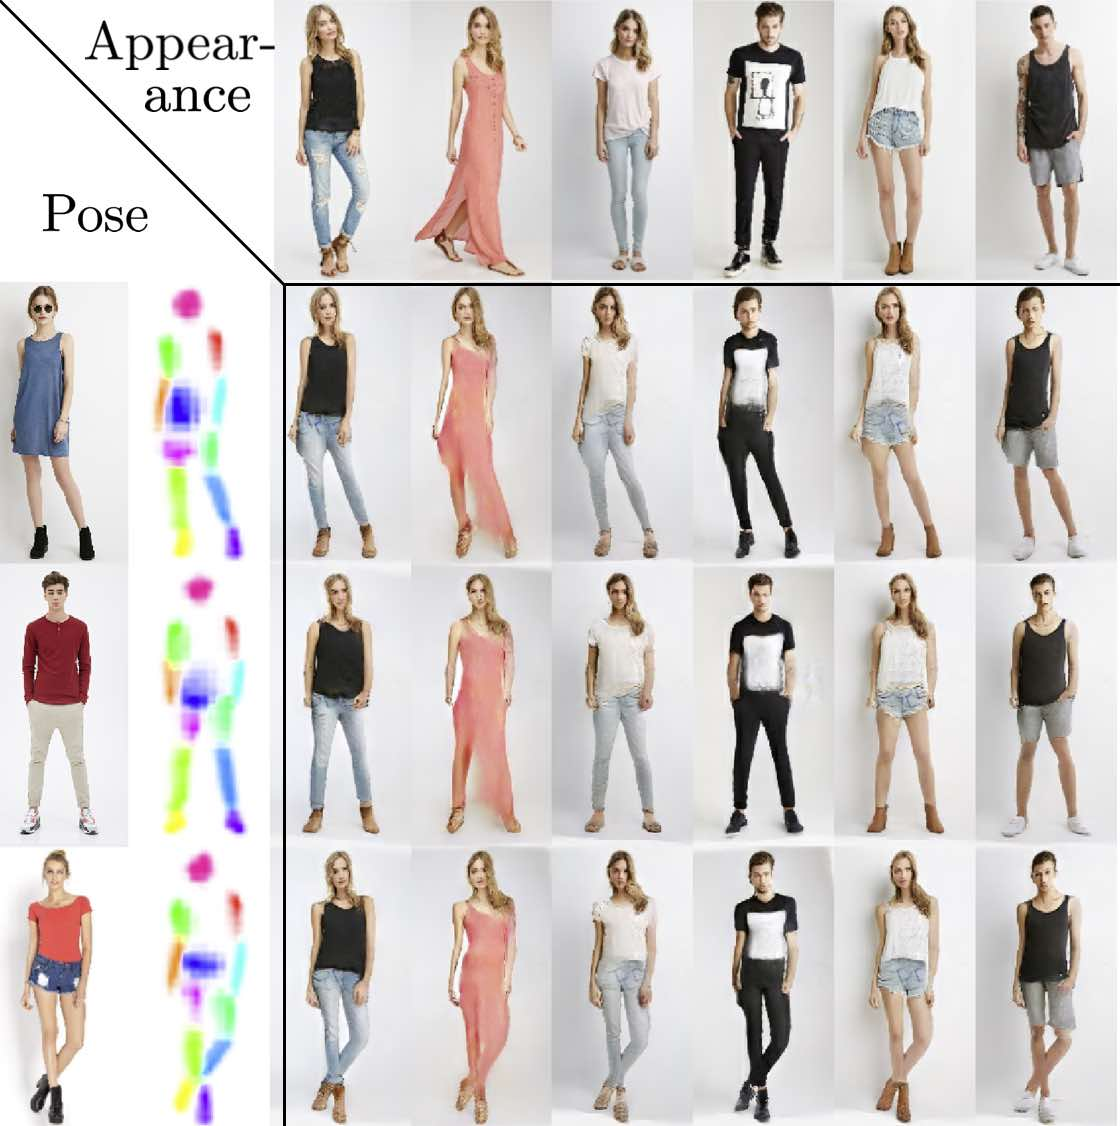
\includegraphics[trim={0cm 0cm 0cm 0cm},clip, width=.5\linewidth]{fig/factor/swappy}
				\caption{Transferring shape and appearance on Deep Fashion. Without annotation the model estimates shape, 2nd column. Target appearance is extracted from images in top row to synthesize images. Note that we trained without image pairs only using synthetic transformations.
				%for training we had no image pairs but only synthetic transformations.
				%without being explicitly trained for this task.
				All images are from the test set.}
				\label{fig:allswaps}
			\end{figure}
		\end{frame}

		\begin{frame}[t]
		\frametitle{Person Re-Identification}
			\begin{table}[htp]
				\centering
				\caption{Mean average precision (mAP) and rank-n accuracy for person re-identification on synthesized images after performing shape/appearance swap. Input images from Deep Fashion test set. Note \cite{esser18} is supervised \wrt shape.}
				\label{tab:reid}
				\begin{tabular}{l|cccr}
					\hline
					& mAP & rank-1 & rank-5 & rank-10 \\ \hline
					VU-Net \cite{esser18} & 88.7\% & 87.5\% & {98.7}\% & {99.5}\% \\
					Ours & {90.3}\% & {89.4}\% &{98.2}\% & {99.2}\% \\ \hline
				\end{tabular}
			\end{table}
		\end{frame}

		\begin{frame}[t]
		\frametitle{Person Re-Identification}
			% TSNE
			\begin{figure}[htp]
				\centering
				\begin{subfigure}{0.49\linewidth}
				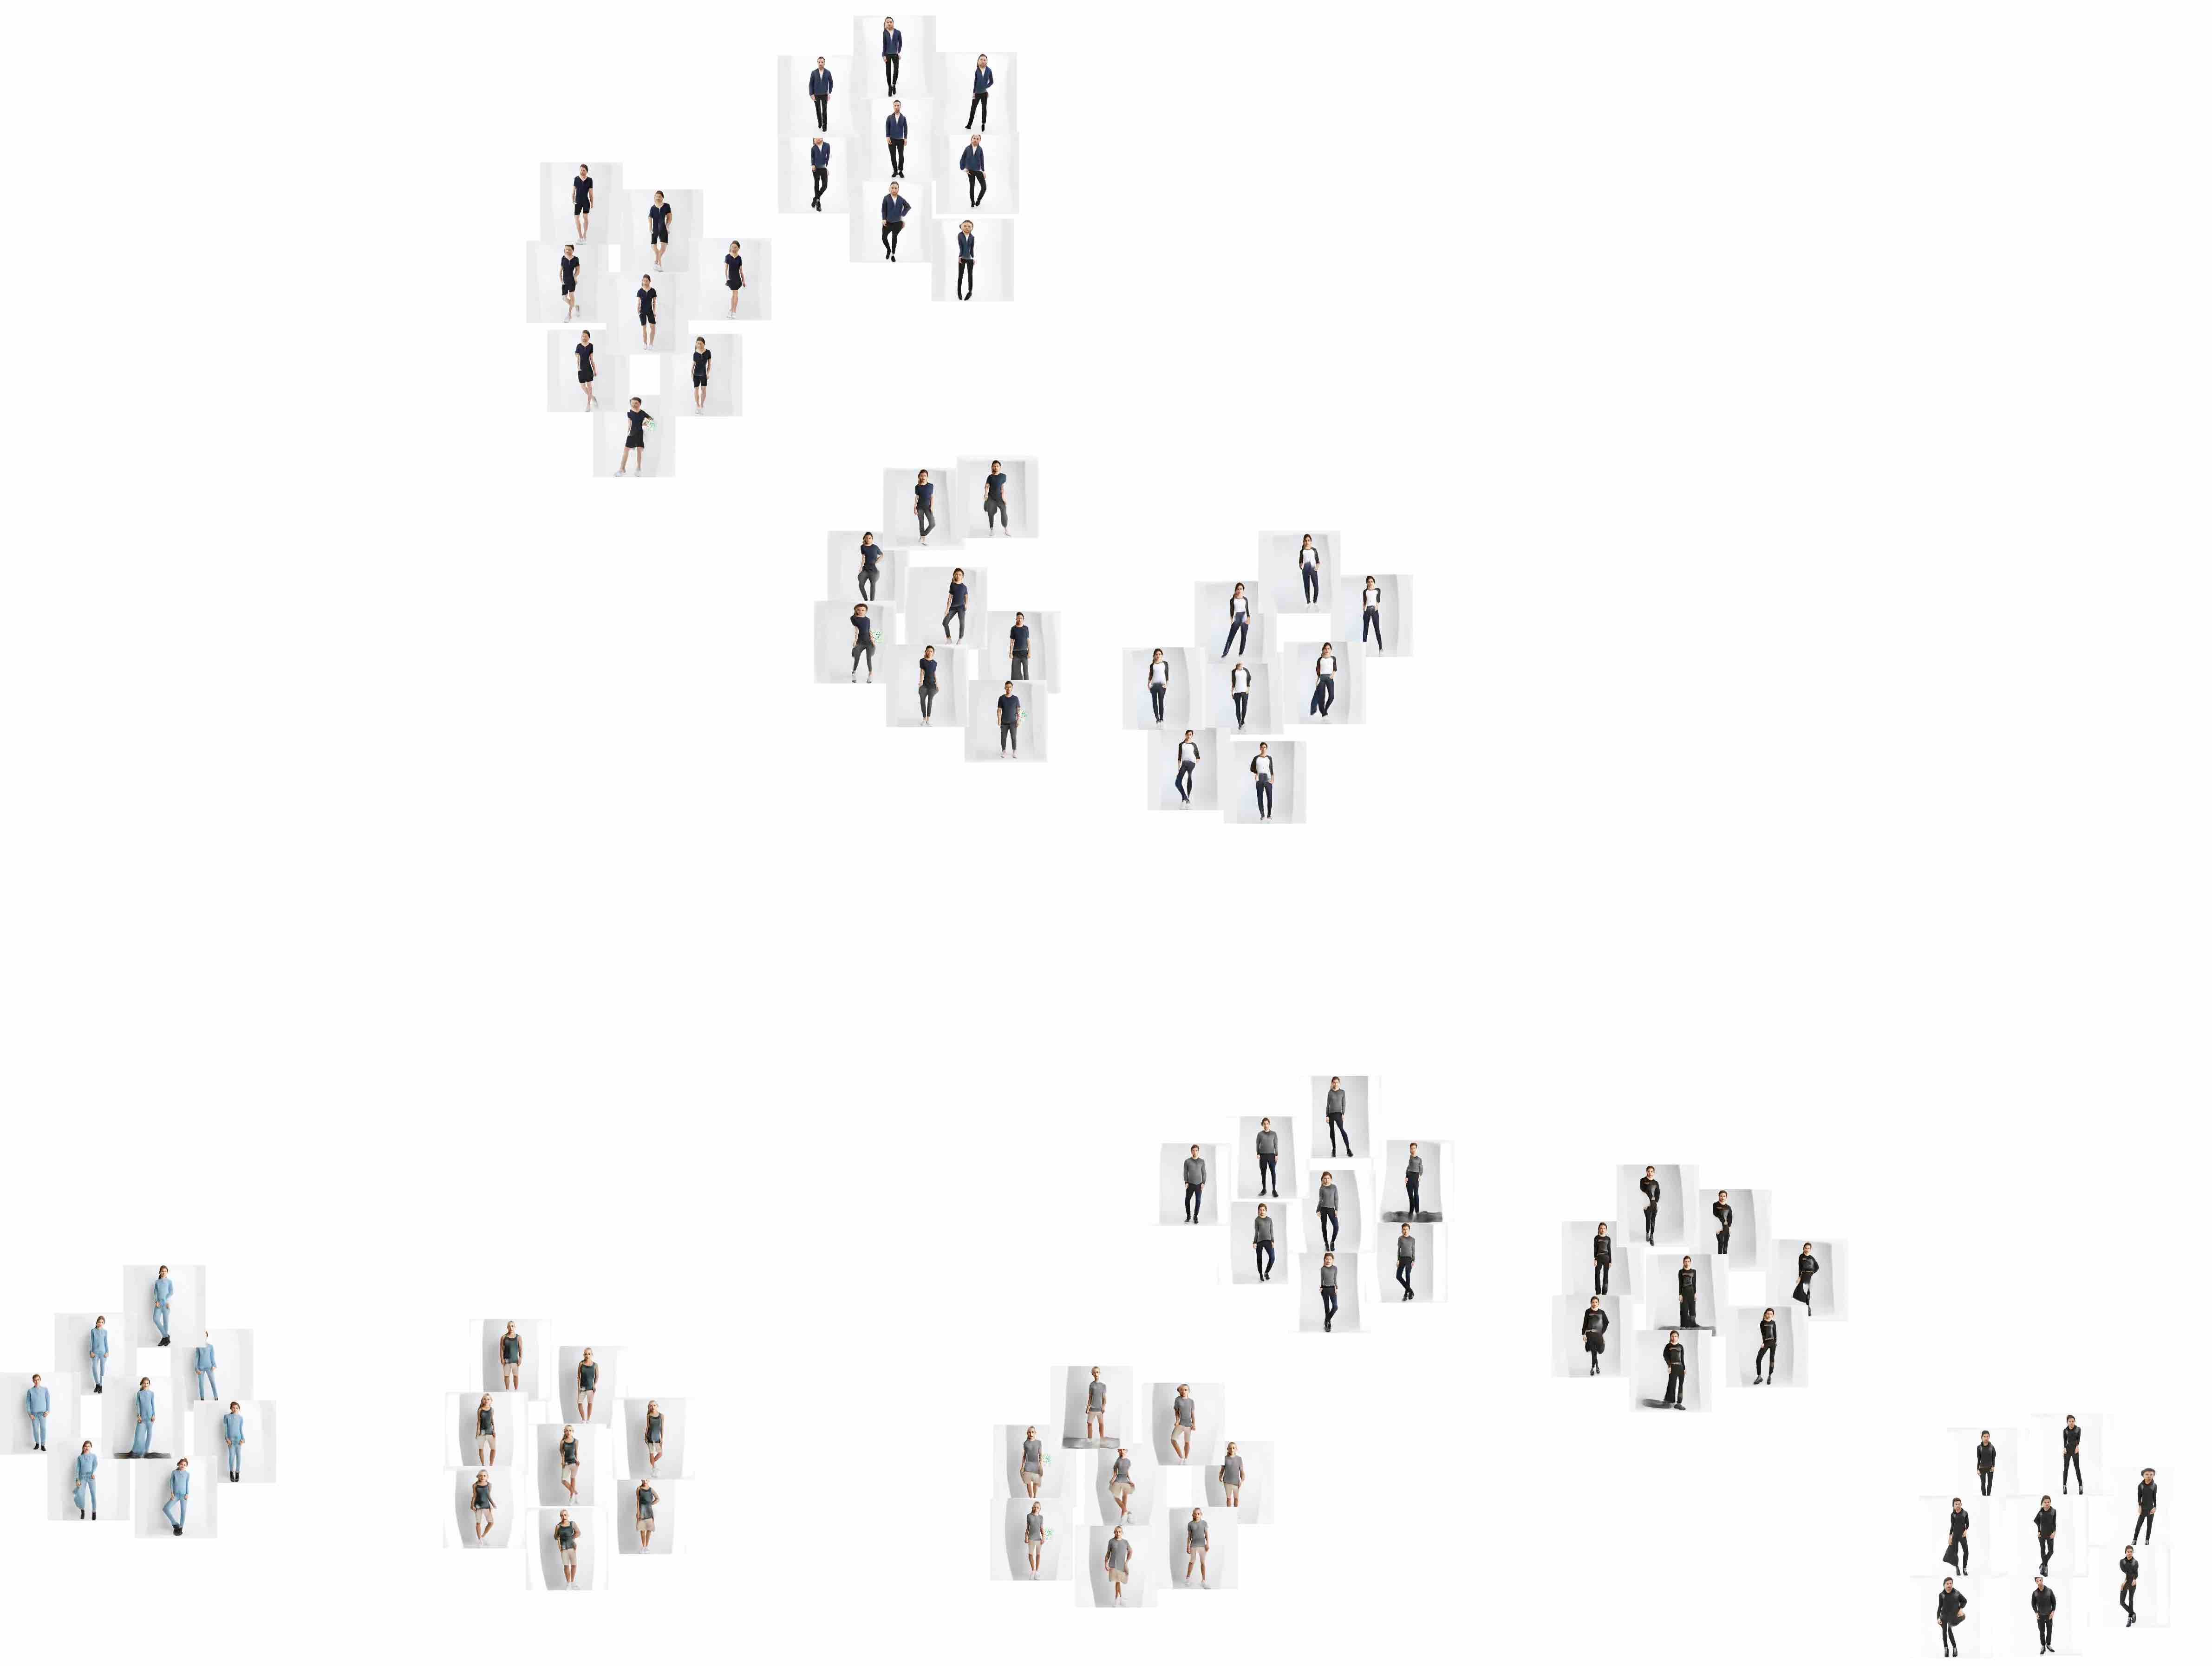
\includegraphics[trim={0cm 0cm 0cm 0cm},clip, width=1.0\linewidth]{fig/factor/tsne_img}
				\end{subfigure}
				\begin{subfigure}{0.49\linewidth}
				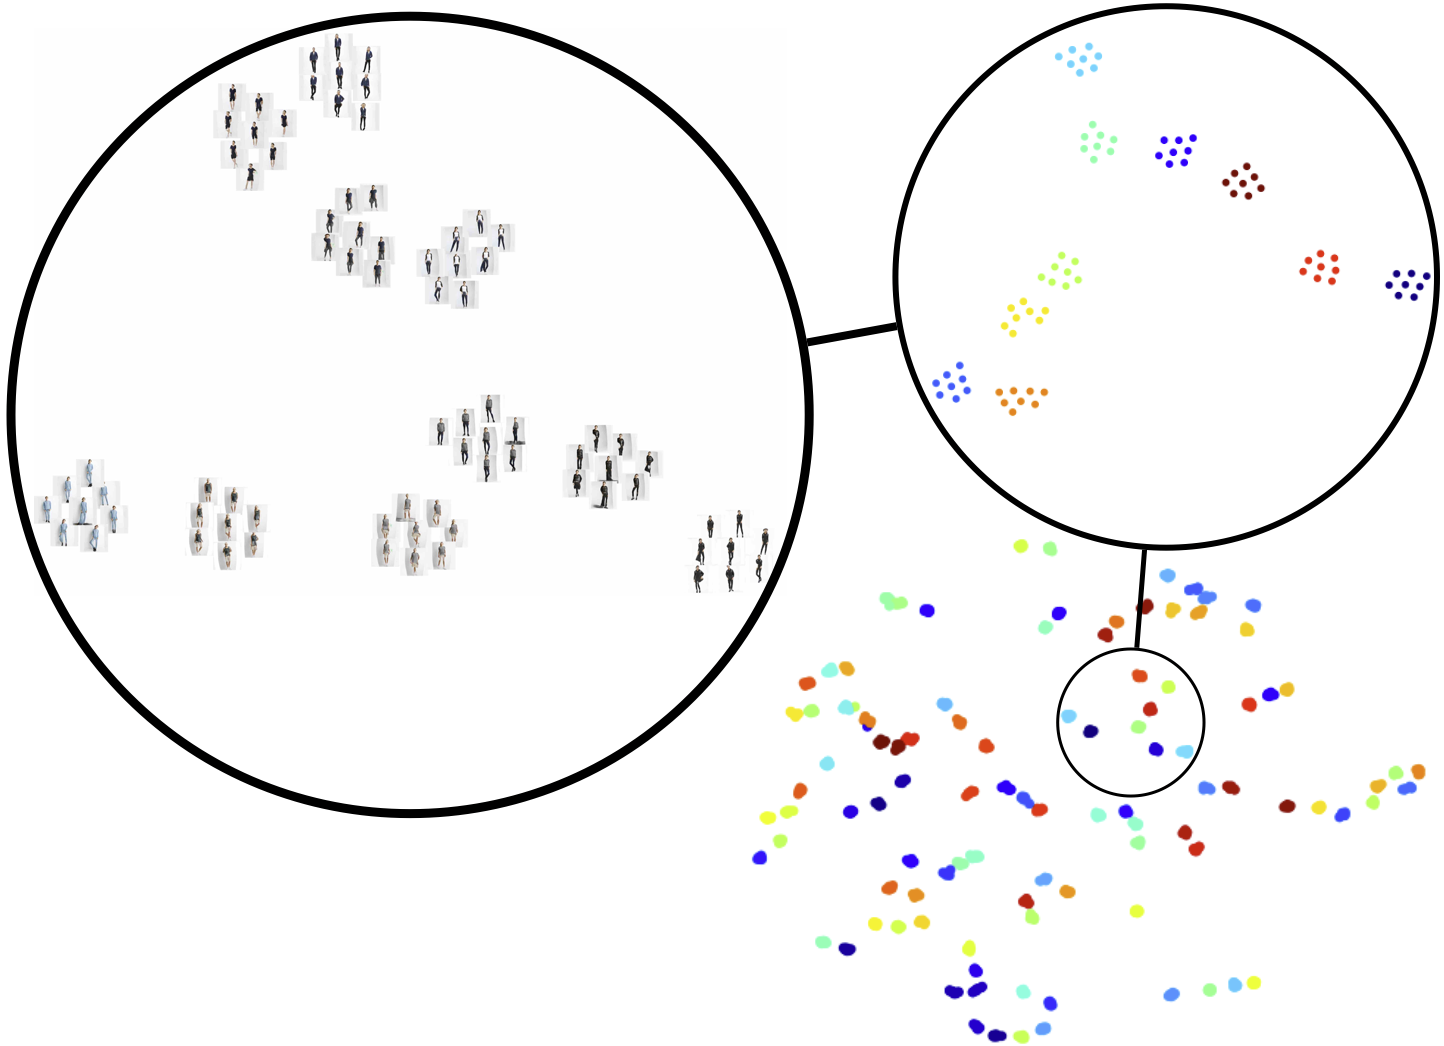
\includegraphics[trim={0cm 0cm 0cm 0cm},clip, width=1.0\linewidth]{fig/factor/tsne_bubble}
				\end{subfigure}
				% \begin{subfigure}{0.49\linewidth}
					% % \begin{subfigure}{0.49\linewidth}
					% 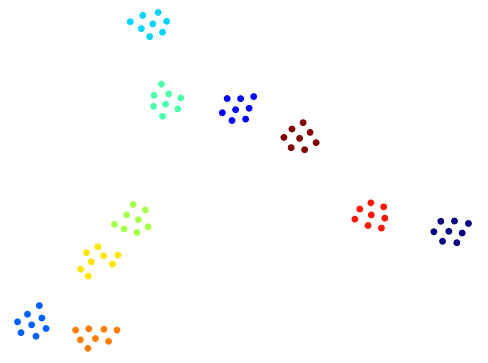
\includegraphics[trim={0cm 0cm 0cm 0cm},clip, width=1.0\linewidth]{fig/factor/tsne10}
					% \end{subfigure}\begin{subfigure}{0.49\linewidth}
					% 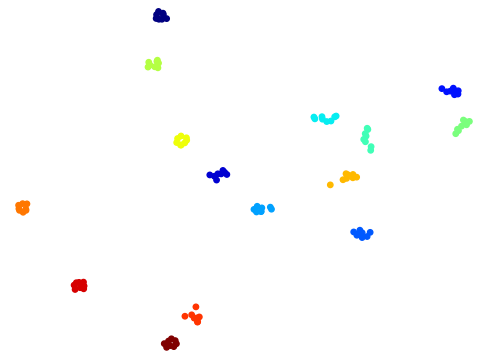
\includegraphics[trim={0cm 0cm 0cm 0cm},clip, width=1.0\linewidth]{fig/factor/tsne15}
					% \end{subfigure}
					% \begin{subfigure}{0.49\linewidth}
					% 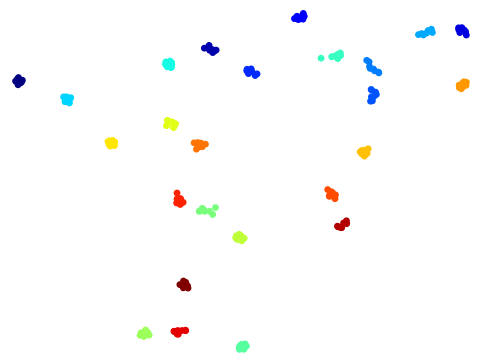
\includegraphics[trim={0cm 0cm 0cm 0cm},clip, width=1.0\linewidth]{fig/factor/tsne20}
					% \end{subfigure}
					% \begin{subfigure}{0.49\linewidth}
					% 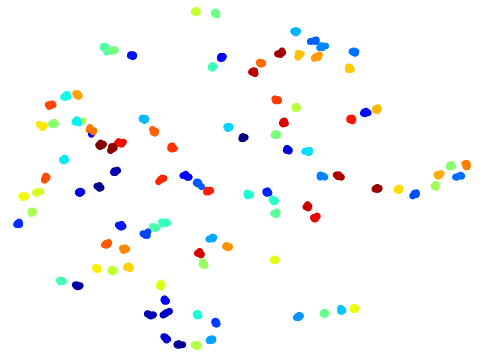
\includegraphics[trim={0cm 0cm 0cm 0cm},clip, width=1.0\linewidth]{fig/factor/tsne100}
					% \end{subfigure}
				% \end{subfigure}
				\caption{Visualization of feature distribution for generated person IDs. (Right) t-SNE (perplexity 16) of 10 generated IDs, (left) color-coded t-SNE (perplexity 12) for 10, 15, 20 and 100 IDs. Each ID has 8 samples. The different IDs are clearly separable, despite variation in pose: Hence, generated appearance is invariant to pose.}
				\label{fig:tsne}
			\end{figure}
		\end{frame}

		\begin{frame}[t]
		\frametitle{Directly Transfer?}
			\begin{table}[htp]
				\centering
				\caption{Mean average precision (mAP) and rank-n accuracy for person re-identification from synthesized to ground truth appearance images after performing shape/appearance swap. When only fine-tuning the ReID algorithm on DeepFashion, results are much worse that when also adjusting to the synthesized images.}
				\label{tab:reiddirect}
				\begin{tabular}{l|cccr}
					\hline
					Fine-tune to: & mAP & rank-1 & rank-5 & rank-10 \\ \hline
					% VU-Net \cite{esser18} & 88.7\% & 87.5\% & {98.7}\% & {99.5}\% \\
					DeepFashion & {17.2}\% & {25.4}\% &{48.8}\% & {60.4}\% \\
					DeepFashion and Synthesized Images& {75.0}\% & {73.8}\% &{89.5}\% & {92.5}\% \\ \hline
				\end{tabular}
			\end{table}
		\end{frame}

		\begin{frame}[t]
		\frametitle{Pose Estimation}
			\begin{table}[htp]
				\centering
				\caption{Percentage of Correct Keypoints (PCK) for pose estimation on shape/appearance swapped generations.\;$\alpha$ is pixel distance divided by image diagonal. Note that \cite{esser18} serves as upper bound, as it uses the groundtruth shape estimates.}
				%shape supervision.}
				\label{tab:pose}
				\begin{tabular}{l|cccr}
					\hline
					$\alpha$ & $2.5\%$ &  $5\%$ & $7.5\%$ & $10\%$ \\ \hline
					VU-Net \cite{esser18} & {95.2}\% & {98.4}\% & {98.9}\% & {99.1}\% \\
					Ours & 85.6\% & 94.2\% &96.5\% & 97.4\% \\ \hline
				\end{tabular}
			\end{table}
		\end{frame}


	\subsection{Disentangling in a Temporal Sequence}
		\begin{frame}[t]
		\frametitle{Video-to-Video Translation}
			\begin{figure}[htp]
				\centering
				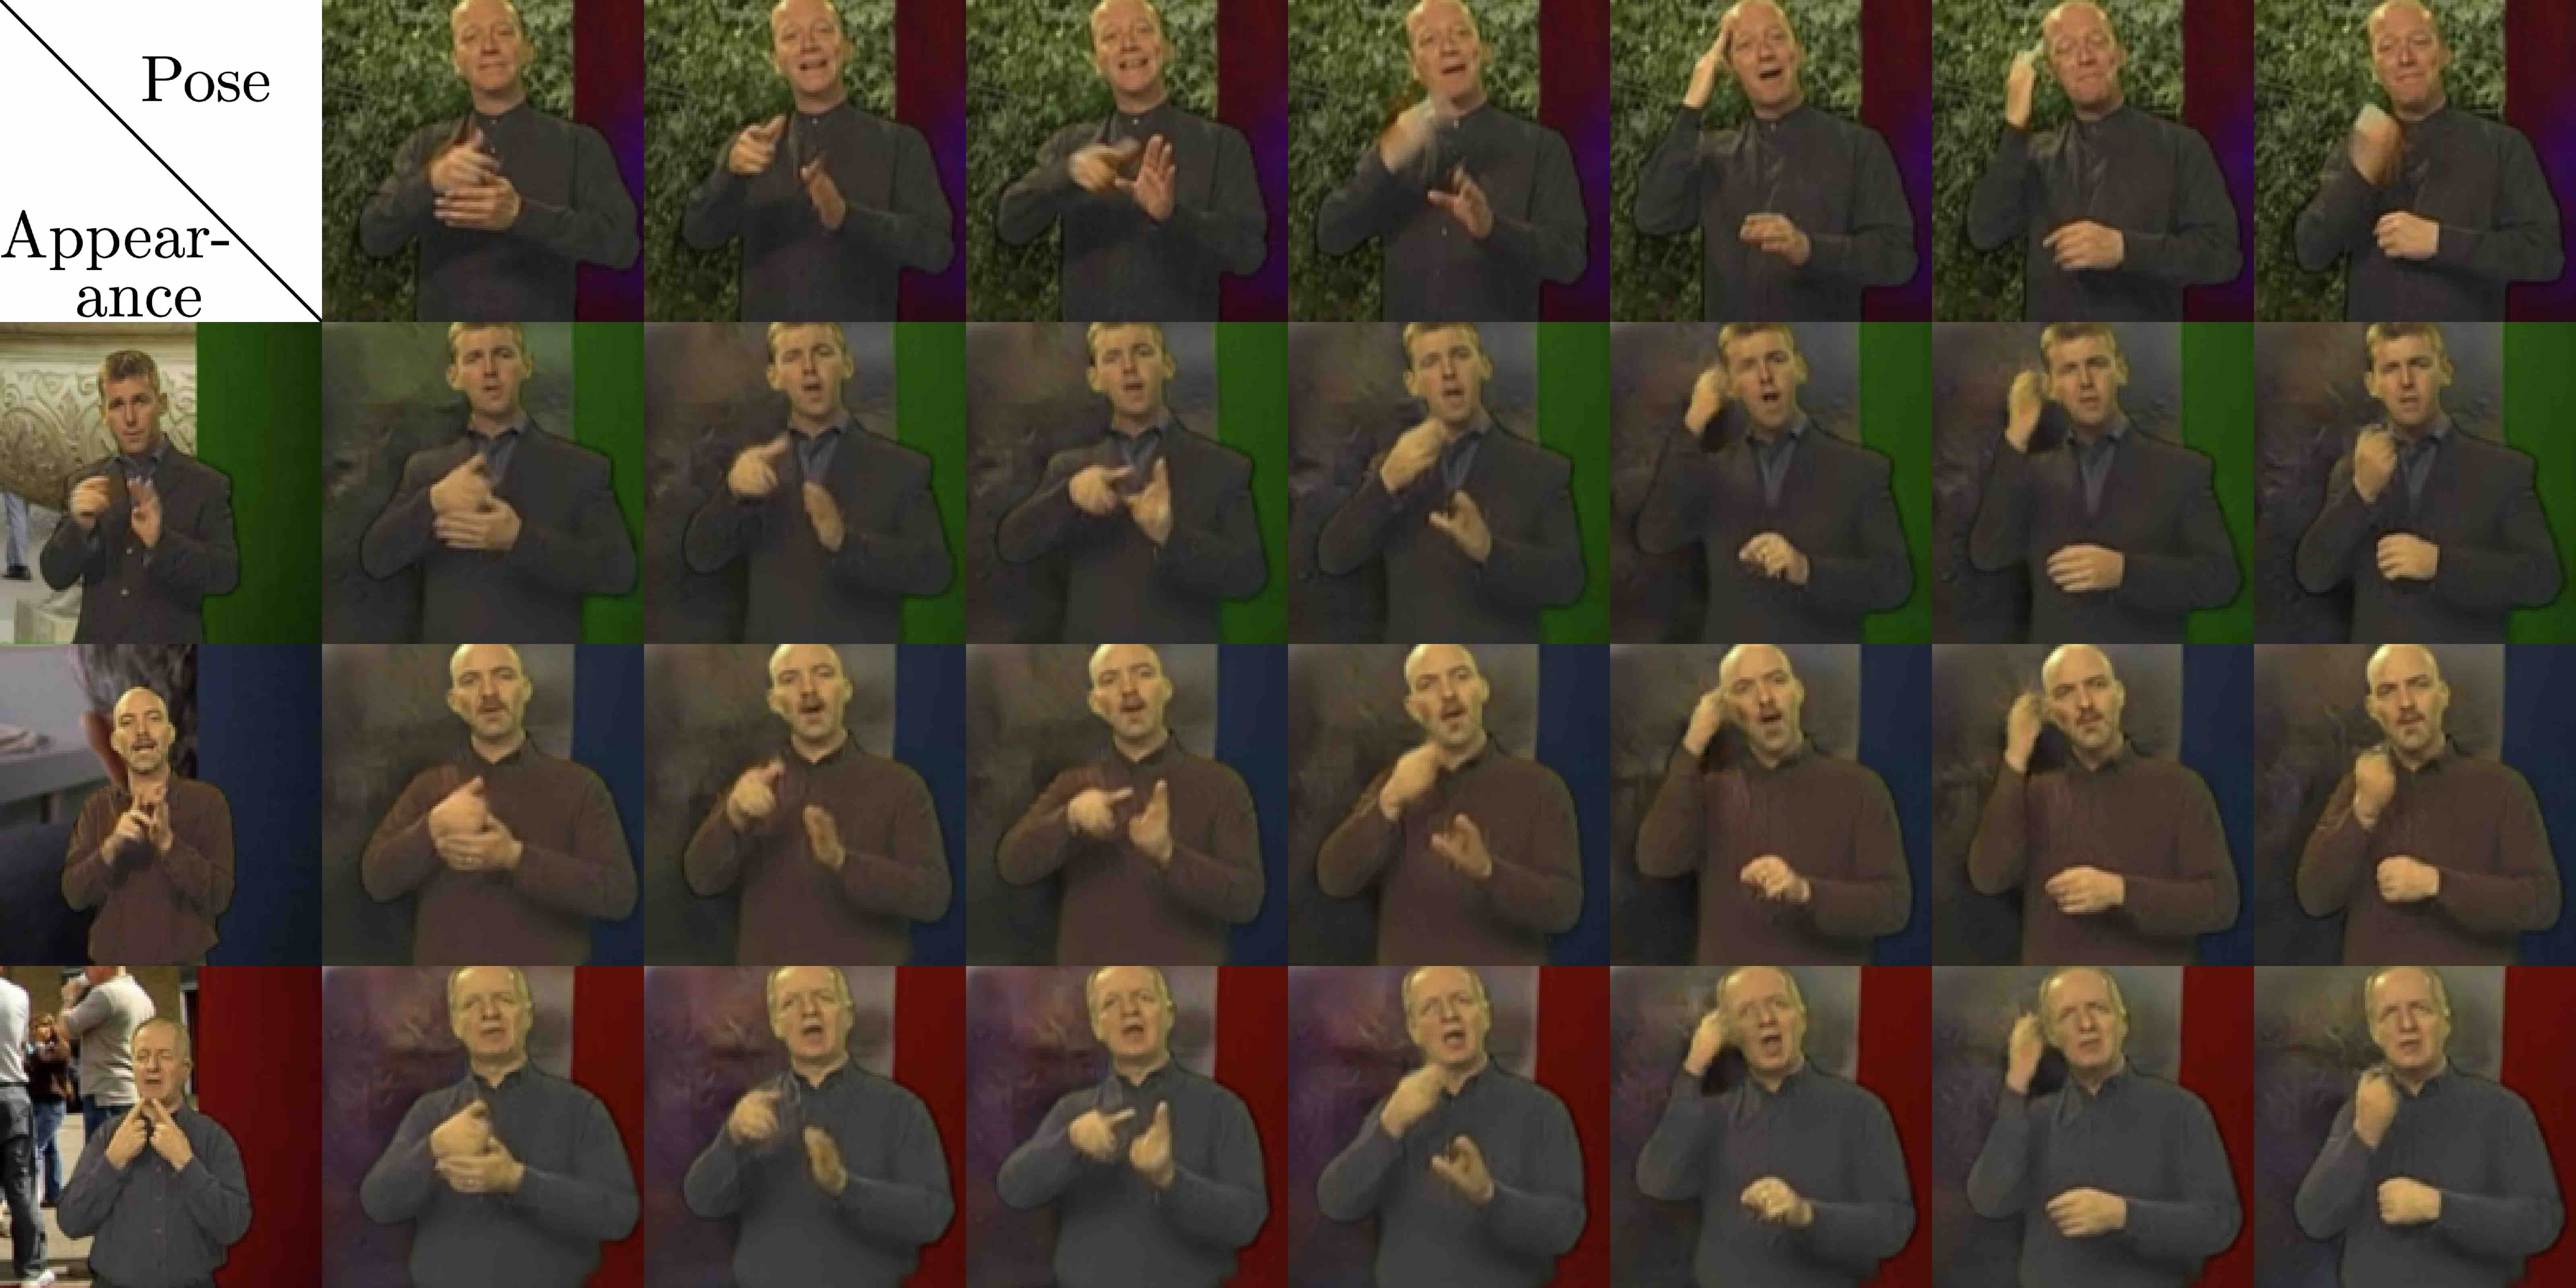
\includegraphics[trim={0cm 0cm 0cm 0cm},clip, width=1.\linewidth]{fig/factor/bbc_arrange}
				\caption{Generation results for conditioning appearances (top row) on pose (bottom, rightmost) on BBCPose.
				% The target appearances are from the train set, while the target pose is from the test set.
				Note that even fine-grained details in shape, such as fingers and facial expression are accurately captured.}
				\label{fig:bbcthumb}
			\end{figure}
		\end{frame}

	\subsection{Disentangling Parts}
		\begin{frame}[t]
		\frametitle{Part-wise Appearance Transfer}
			% PART SWAPS
			\begin{figure}[htp]
				\begin{subfigure}{0.49\linewidth}
				\centering
				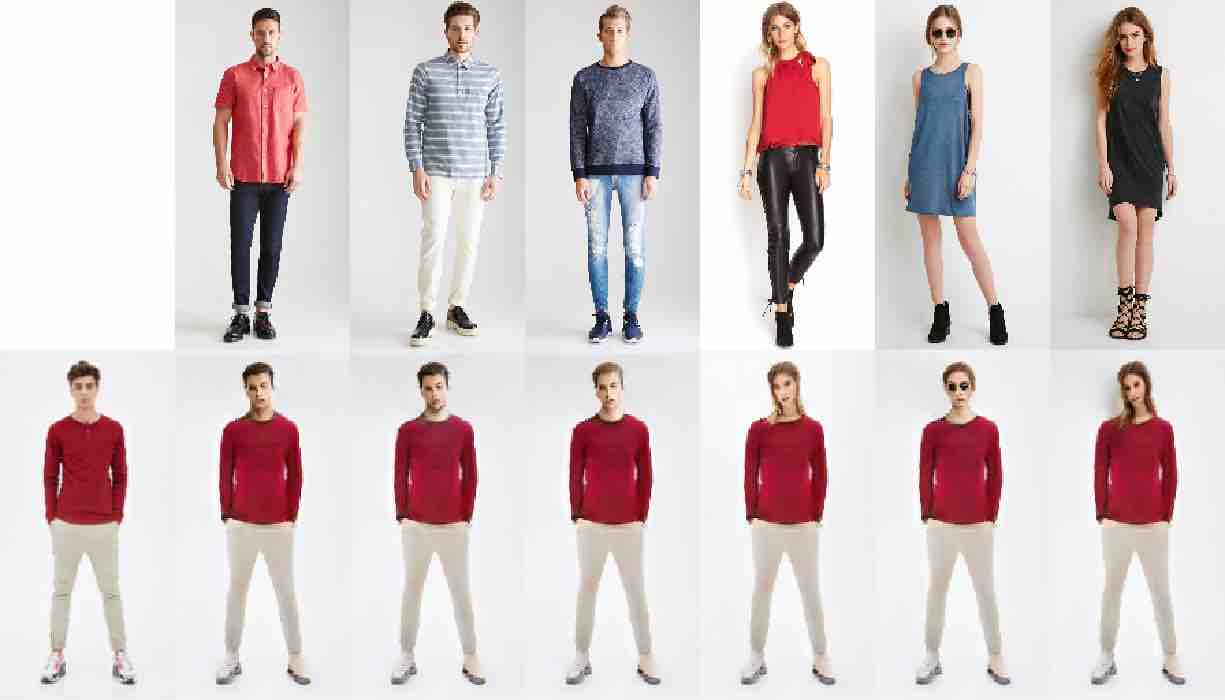
\includegraphics[trim={0cm 0cm 0cm 0cm},clip, width=1.\linewidth]{fig/factor/part6_01}\caption{}
				\label{fig:part3_00}
				\end{subfigure}
				\begin{subfigure}{0.49\linewidth}
				\centering
				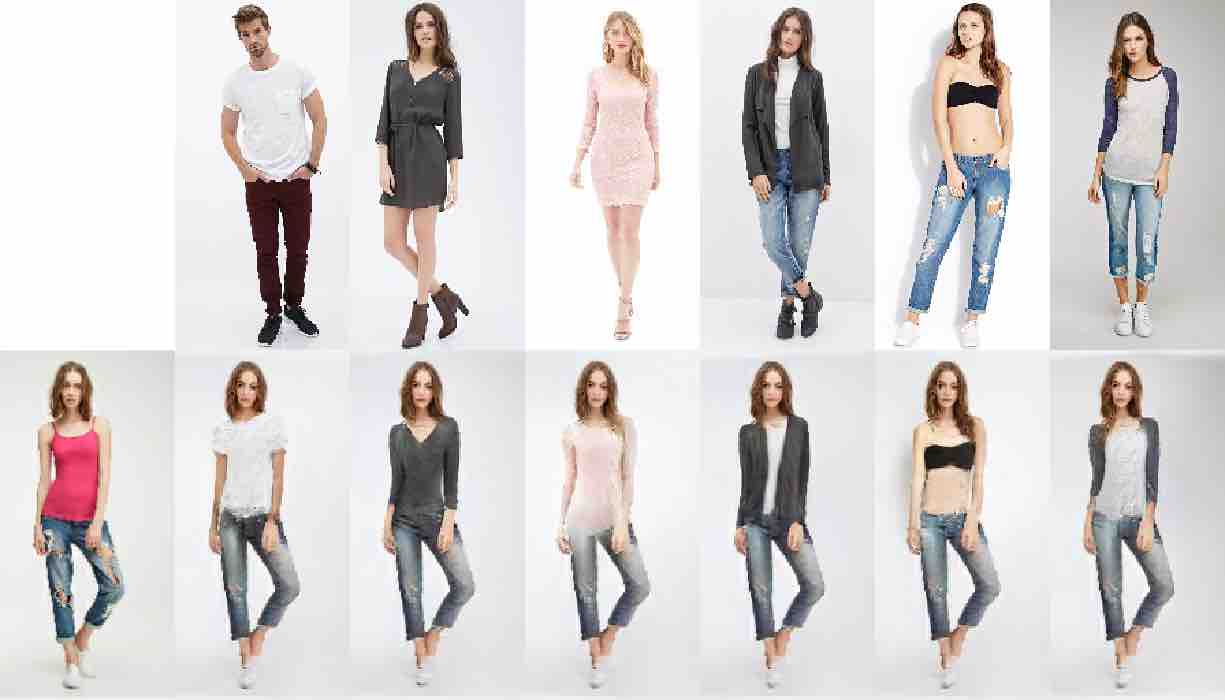
\includegraphics[trim={0cm 0cm 0cm 0cm},clip, width=1.\linewidth]{fig/factor/part6_10}\caption{}
				\label{fig:part3_11}
				\end{subfigure}
				\begin{subfigure}{0.49\linewidth}
				\centering
				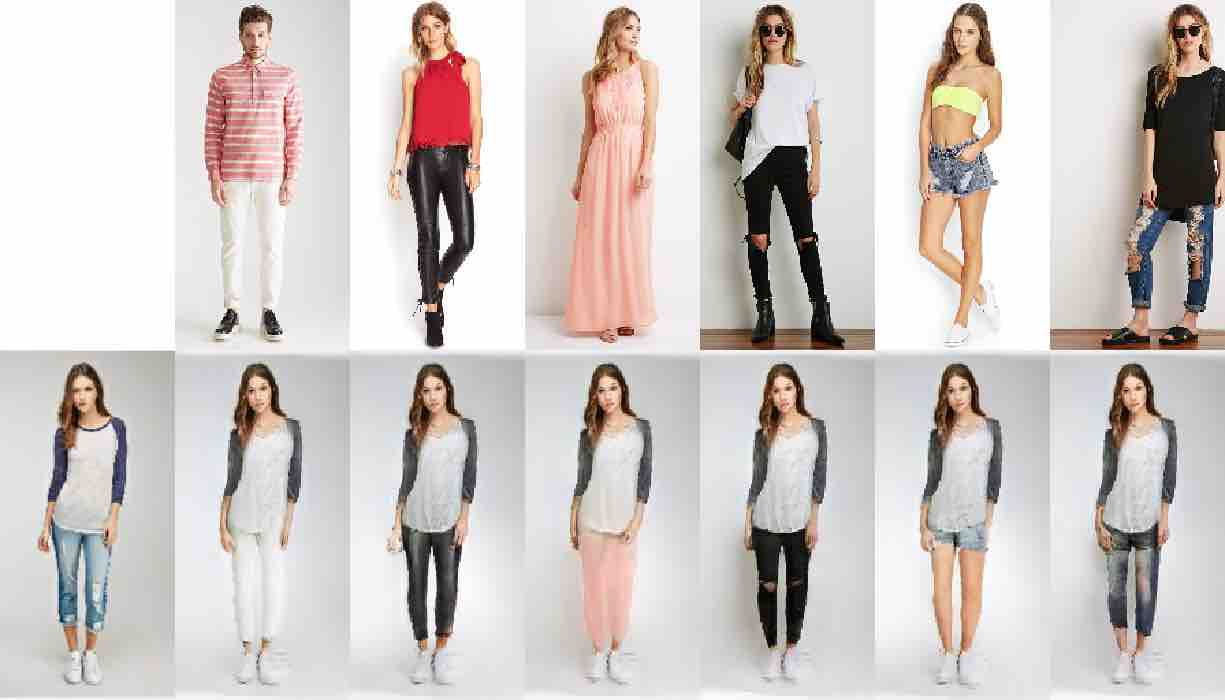
\includegraphics[trim={0cm 0cm 0cm 0cm},clip, width=1.\linewidth]{fig/factor/part6_21}\caption{}
				\label{fig:part3_21}
				\end{subfigure}
				\begin{subfigure}{0.49\linewidth}
				\centering
				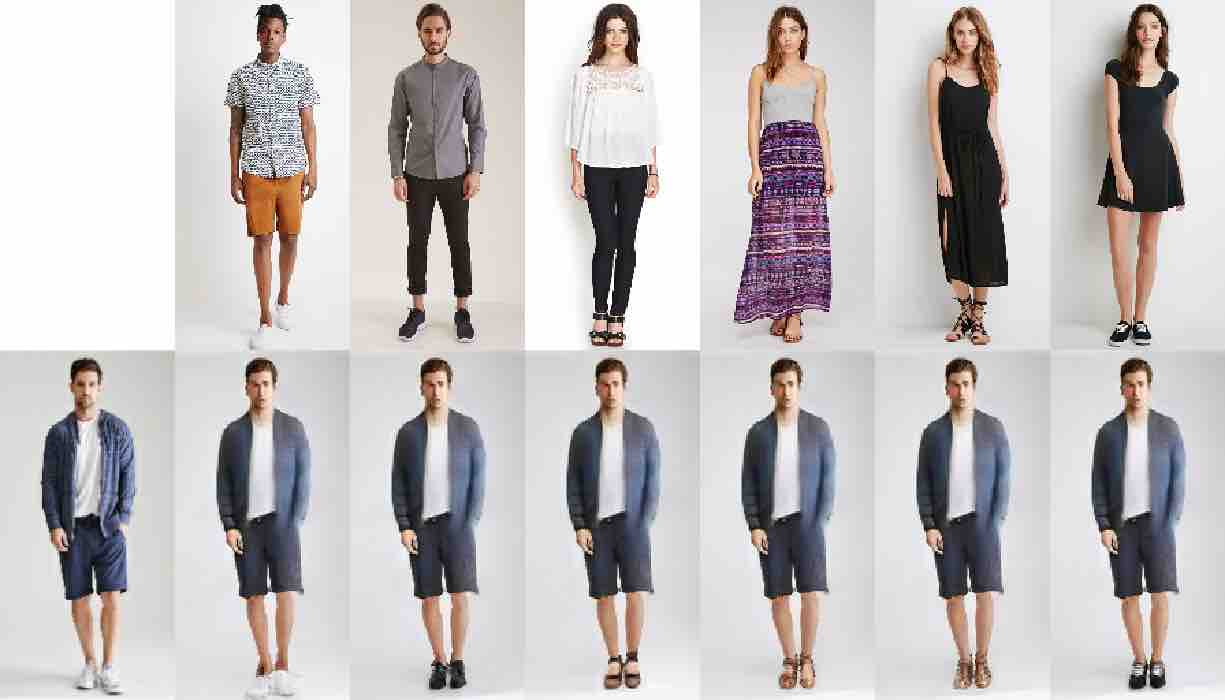
\includegraphics[trim={0cm 0cm 0cm 0cm},clip, width=1.\linewidth]{fig/factor/part6_30}\caption{}
				\label{fig:part3_30}
				\end{subfigure}
				\caption{Swapping part appearance on Deep Fashion. Appearances can be exchanged for parts individually and without altering shape. We show part-wise swaps for (a) head (b) torso (c) legs, (d) shoes. All images are from the test set.}
				\label{fig:partswaps}
			\end{figure}
		\end{frame}

		\begin{frame}[t]
		\frametitle{Part-wise Shape Changes}
			\begin{figure}[htp]
				\centering
				\begin{subfigure}{1.\linewidth}
					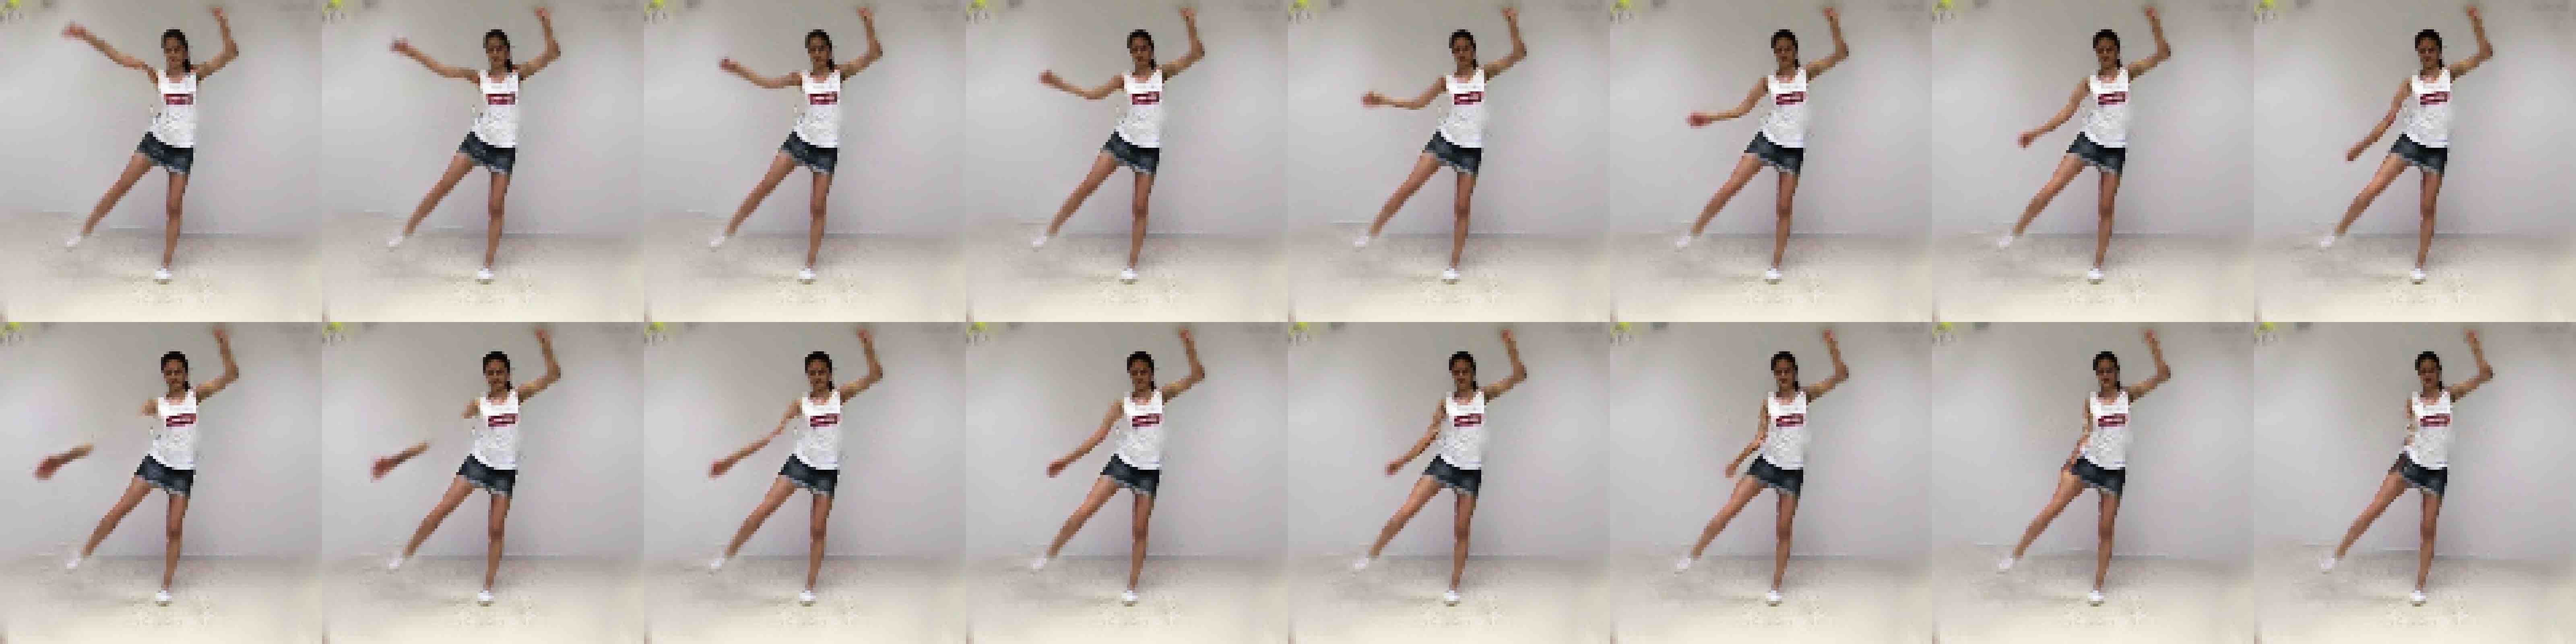
\includegraphics[trim={0cm 0cm 0cm 0cm},clip, width=1.0\linewidth]{fig/factor/8arm}\caption{}
				\end{subfigure}
				\begin{subfigure}{1.\linewidth}
					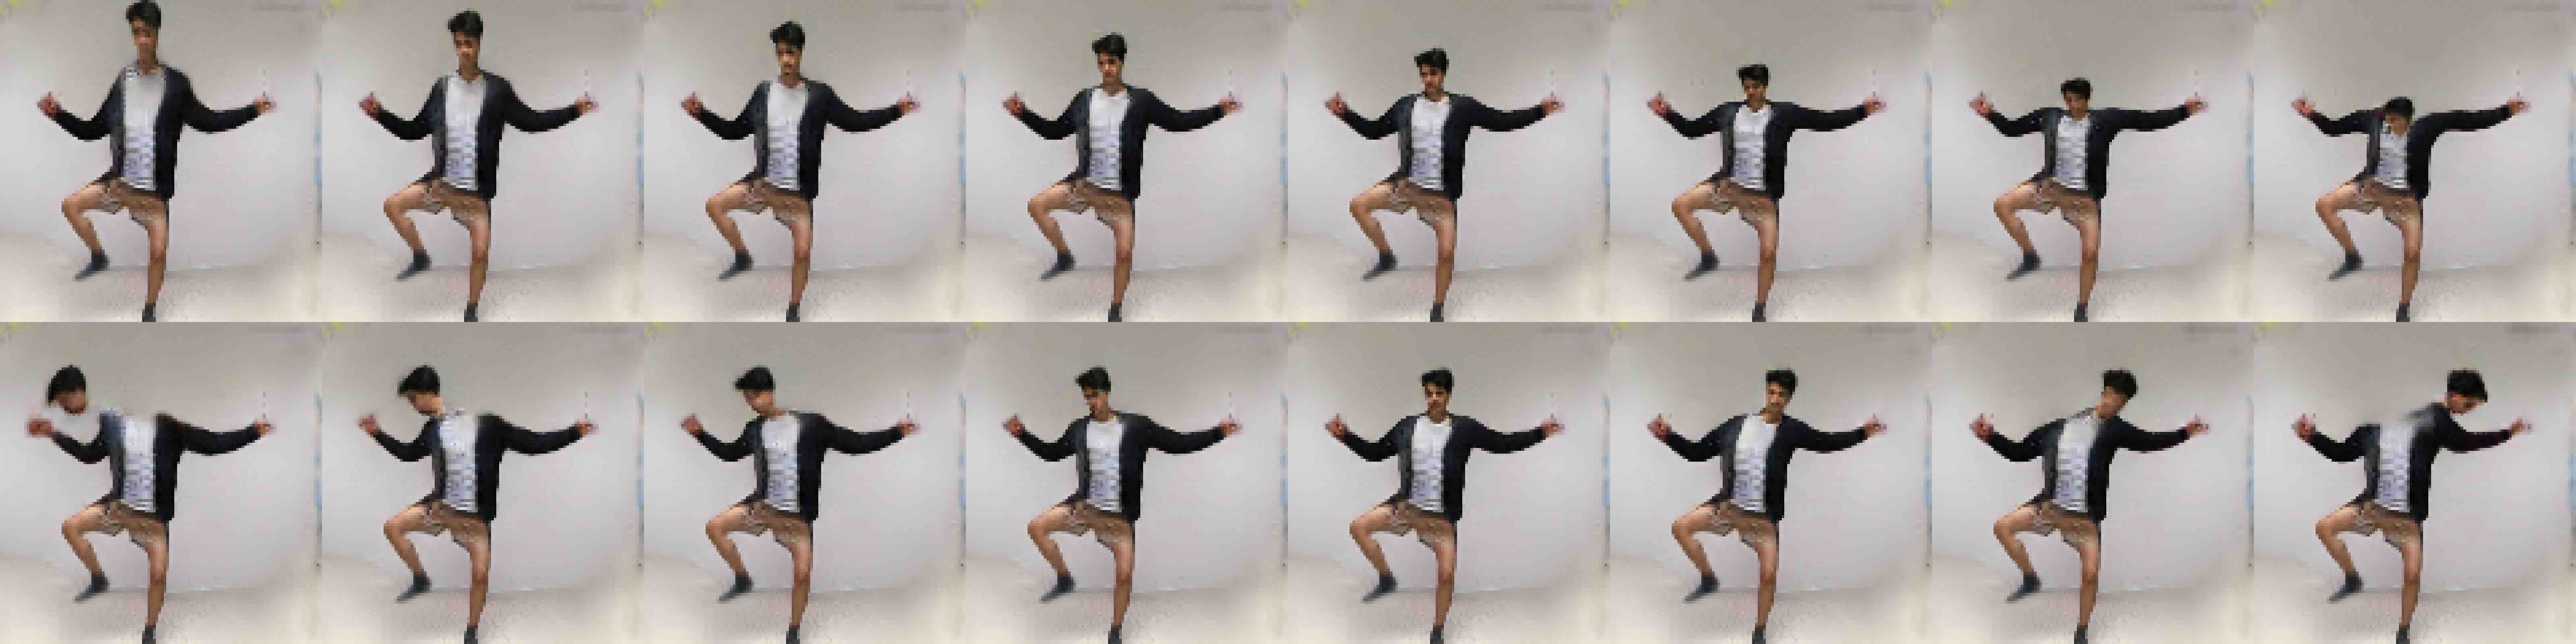
\includegraphics[trim={0cm 0cm 0cm 0cm},clip, width=1.0\linewidth]{fig/factor/8head}\caption{}
				\end{subfigure}
				\caption{Moving individual body landmarks for conditional generation: (a) arm (b) head.}
				\label{fig:movekp}
			\end{figure}
		\end{frame}

\section{Conclusion}
	\begin{frame}[t]
	\frametitle{Future Work}
		\begin{itemize}
			\item Model better
			\item Transform better
		\end{itemize}
	\end{frame}


	\begin{frame}[t]
	\frametitle{Final Thoughts}
		\begin{itemize}
			\item Causality is important!
			\item Interaction is crucial!
			\item Rethink Disentangling  % model or discover relations
		\end{itemize}
	\end{frame}

